\documentclass{article}
\usepackage[utf8]{inputenc}
\usepackage{graphicx} % Required for inserting images
\usepackage{hyperref}
\usepackage{fvextra}
\usepackage{tikz}
\usepackage{amsmath}
\usepackage{tcolorbox}
\usepackage{multirow}
\usepackage[margin=2cm]{geometry} % <-- AÑADE ESTA LÍNEA
\usetikzlibrary{shapes, arrows, positioning, shapes.geometric}
\usetikzlibrary{positioning, arrows.meta, shapes.geometric}
\usetikzlibrary{shadows.blur}
\usepackage{pgf-pie} % Para el gráfico de torta
\DefineVerbatimEnvironment{Prompt}{Verbatim}{breaklines=true, breakanywhere=true, breaksymbolleft={},   % remove left arrow
  breaksymbolright={}}
\title{IIC3694 - Informe Desafío de Investigación}
\author{Sebastián Burgos, Gonzalo Fernández, Nicolás Sumonte}
\date{Octubre 2025}
\begin{document}
\maketitle

\section{Introducción}

Este trabajo construye un dataset cultural basado en grafos de conocimiento en el dominio médico para evaluar brechas de conocimiento regional en modelos de lenguaje de frontera. El dataset, estructurado como tripletas $\langle$entidad, relación, valor$\rangle$, contiene 78.208 tripletas sobre medicamentos, enfermedades, exámenes de laboratorio y artículos científicos latinoamericanos, junto con 76.234 tripletas de fuentes estadounidenses para comparación. La evaluación de tres modelos (Qwen 2.5 7B, Llama 3.1 8B, Mistral 0.3 7B) sobre más de 200.000 instancias revela diferencias significativas en cómo representan conocimiento médico latinoamericano versus anglosajón, evidenciando sesgos lingüísticos y geográficos que varían sustancialmente entre modelos. El grafo de conocimiento y código están disponibles en \url{https://github.com/VadokDev/grafo-conocimiento-medico}.

\section{Descripción del dataset}

El dataset fue elaborado a partir de información sobre medicamentos, enfermedades, pruebas de laboratorio y de entidades relevantes en artículos científicos latinoamericanos (en su mayoría chilenos) del área de la salud.

\subsection{Recolección de información}

La construcción del dataset parte desde la recolección de las fuentes con las entidades y el conocimiento sobre ellas a trabajar. Para los medicamentos se realizó \textit{scraping} sobre el sitio web de Medline en español \cite{medlineplus}, de donde se recopiló la información de 1.948 medicamentos, los cuales quedaron en sus respectivos archivos de texto. Por ejemplo, para el medicamento Abacavir \cite{medlineplus_abacavir}, se aprecia en el apéndice ~\ref{app:abacavir}. La información obtenida contempla el uso, las precauciones e indicaciones generales para cada medicamento, aunque algunas entradas de medicamentos cuentan con menos información que otras, no le resta relevancia a los datos obtenidos.

Para las pruebas o exámenes de laboratorio se realizó el mismo procedimiento también desde el sitio web de Medline en español \cite{medlineplus}, resultando en un total de 297 pruebas de laboratorio. La información general es sobre qué es la prueba, para qué se usa, riesgos, entre otros.

Para las enfermedades se utilizó el dataset \texttt{enfermedades-wiki-marzo-2024} \cite{enfermedades_wiki}. Este dataset contiene información de 945 enfermedades obtenidas de Wikipedia en español \cite{wikipedia_es}. Cada enfermedad tiene un resumen de lo que es, su tratamiento y su diagnóstico.

Para los artículos científicos latinoamericanos se utilizó SciELO \cite{scielo} para su búsqueda. Se implementó un scraper para buscar en revistas médicas relevantes. Los artículos resultantes son de investigación, de revisión o de reporte de caso clínico. En total se recopilaron 1.742 artículos de Latinoamérica, en su mayoría chilenos.

\subsection{Creación de tripletas}

Para los datasets de medicamentos, pruebas de laboratorio y enfermedades se determinó cada archivo/objeto como la entidad. Es decir, cada medicamento o cada enfermedad en sí es la entidad. Luego, para la creación de las tripletas se implementó un script que buscara relaciones y sus valores. Este script usa Procesamiento de Lenguaje Natural (NLP), a través de la librería spaCy \cite{spacy}. Los resultados obtenidos no fueron del todo satisfactorios, ya que en general las relaciones encontradas eran correctas, pero los valores no; por lo tanto, de este trabajo sólo se conservaron las relaciones, mas no las tripletas generadas. Además, se agregaron y/o editaron relaciones en la medida en que el equipo lo consideró pertinente.

Entonces, realizamos un cambio de enfoque y utilizamos LLMs para determinar los valores de las relaciones determinadas para cada entidad. Al hacer pruebas de concepto, este determinaba sustancialmente de mejor manera los valores. En específico, ocupamos \texttt{gpt-4o-mini} de OpenAI. Una ilustración del procedimiento se puede apreciar en la Figura \ref{fig:pipeline-tripletas}. Como ejemplo, el prompt usado para los medicamentos es:

\begin{tcolorbox}[
    colback=blue!5!white,
    colframe=blue!75!black,
    title=Prompt de Extracción de Información Médica,
    fonttitle=\bfseries,
    rounded corners,
    arc=4mm,
    boxrule=1pt,
    left=5pt,
    right=5pt,
    top=5pt,
    bottom=5pt
]
Analiza el siguiente texto sobre el medicamento ``\{nombre\_medicamento\}'' (si el nombre del medicamento tiene caracteres especiales, arréglalos).

Extrae información factual únicamente relacionada con las siguientes categorías y devuélvela en formato JSON como una lista de tripletas con los campos: ``entidad'', ``relacion'' y ``valor''.

\textbf{Las relaciones válidas son:}
\begin{itemize}
    \item \texttt{contraindicado\_en} (Advertencia)
    \item \texttt{trata} (¿Para cuáles condiciones o enfermedades se prescribe este medicamento?)
    \item \texttt{uso} (¿Cómo se debe usar este medicamento?)
    \item \texttt{se\_administra\_via} (¿Por qué vía se administra el medicamento?)
    \item \texttt{otro\_uso} (¿Qué otro uso se le da a este medicamento?)
    \item \texttt{precaucion} (¿Cuáles son las precauciones especiales que debo seguir?)
    \item \texttt{dieta} (¿Qué dieta especial debo seguir mientras tomo este medicamento?)
    \item \texttt{olvido} (¿Qué tengo que hacer si me olvido de tomar una dosis?)
    \item \texttt{efecto\_secundario} (¿Cuáles son los efectos secundarios que podría provocar este medicamento?)
    \item \texttt{almacenamiento} (¿Cómo debo almacenar este medicamento?)
    \item \texttt{sobredosis} (¿Qué debo hacer en caso de una sobredosis?)
    \item \texttt{marca\_comercial} (Marcas comerciales)
\end{itemize}

Si una categoría tiene múltiples valores, crea una tripleta separada para cada valor.

Si alguna categoría no tiene información en el texto, simplemente no la incluyas.

Si encuentras una nueva relación que no está en la lista, inclúyela igualmente.

Usa lenguaje conciso para el valor y evita duplicados.

\textbf{Texto:}

\texttt{"""\{texto\}"""}

\textbf{Ejemplo de salida:}

\texttt{[} \\
\texttt{~~\{\{"entidad": "Baclofeno", "relacion": "trata", "valor": "espasticidad muscular causada por esclerosis múltiple"\}\},} \\
\texttt{~~\{\{"entidad": "Baclofeno", "relacion": "efecto\_secundario", "valor": "mareos"\}\},} \\
\texttt{~~\{\{"entidad": "Baclofeno", "relacion": "uso", "valor": "solución oral, tres veces al día"\}\}} \\
\texttt{]}
\end{tcolorbox}
En el caso de los artículos científicos, se le pidió al LLM (\texttt{gpt-4o-mini}) determinar la tripleta en su totalidad. Esto, ya que en los artículos se presentan varias entidades y la estructura es más libre, por lo que también hay varias relaciones. Entonces, se implementó el siguiente prompt:
\begin{tcolorbox}[
    colback=green!5!white,
    colframe=green!65!black,
    title=Prompt de Extracción de Información de Artículos Científicos,
    fonttitle=\bfseries,
    rounded corners,
    arc=4mm,
    boxrule=1pt,
    left=5pt,
    right=5pt,
    top=5pt,
    bottom=5pt
]
Analiza el siguiente texto de un artículo científico latinoamericano titulado ``\{nombre\_articulo\}''.

Tu tarea es identificar y extraer información factual en forma de tripletas $\langle$entidad, relación, valor$\rangle$.

\textbf{Instrucciones:}
\begin{enumerate}
    \item Identifica conceptos, organizaciones, instituciones, fenómenos, enfermedades, tratamientos, métodos o hallazgos relevantes como \textbf{entidades}.
    \item Identifica \textbf{relaciones explícitas o implícitas} entre entidades, usando verbos o frases que indiquen vínculo (por ejemplo: ``causa'', ``afecta a'', ``describe'', ``pertenece a'', ``investiga'', ``utiliza'', ``evalúa'', ``publica'', ``dirigido por'').
    \item Resume los valores de forma breve y clara.
    \item \textbf{No} incluyas datos específicos del artículo, como numéricos específicos, tamaño de muestra, porcentajes o resultados experimentales exactos.
    \item Usa lenguaje conciso, factual y evita duplicados.
    \item Si una entidad tiene múltiples relaciones o valores, genera una tripleta separada para cada uno.
    \item Devuelve la salida \textbf{solo en formato JSON}, sin texto adicional.
\end{enumerate}

\textbf{Texto:}

\texttt{"""\{texto\}"""}

\textbf{Ejemplo de salida:}

\texttt{[} \\
\texttt{~~\{\{"entidad": "Ministerio de Salud de Chile (MINSAL)", "relacion": "suministra", "valor": "vacunas"\}\},} \\
\texttt{~~\{\{"entidad": "Universidad Austral de Chile", "relacion": "es un", "valor": "lugar de estudio"\}\},} \\
\texttt{~~\{\{"entidad": "estrés académico", "relacion": "causa", "valor": "trastornos emocionales en universitarios"\}\},} \\
\texttt{]}
\end{tcolorbox}

\begin{figure}[h]
\centering
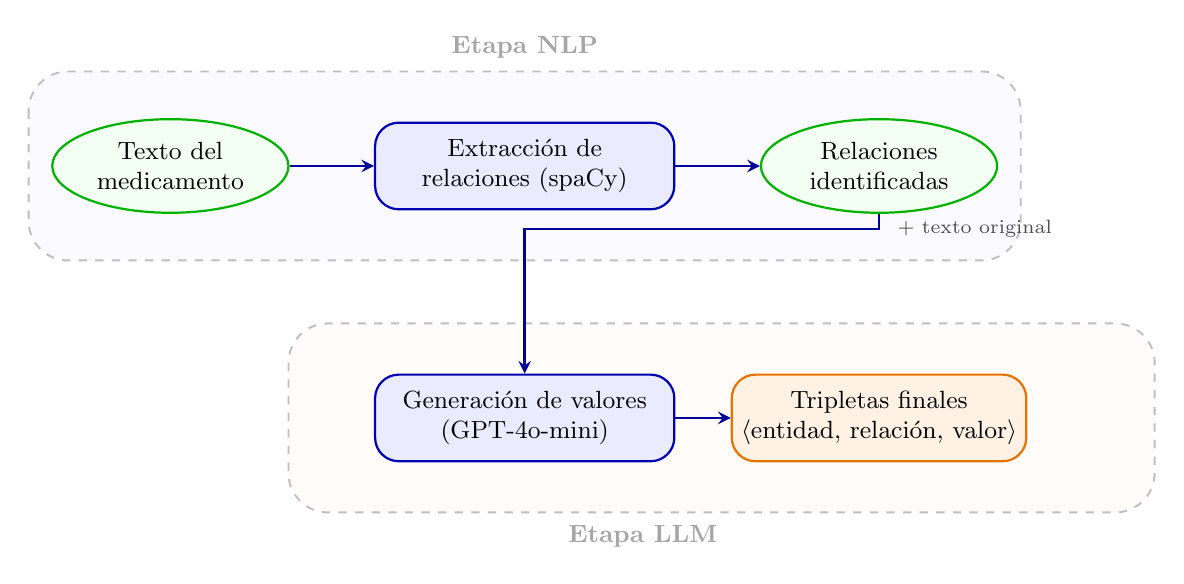
\begin{tikzpicture}[
    node distance=2.8cm and 3cm,
    every node/.style={align=center, font=\small},
    data/.style={ellipse, draw=green!70!black, fill=green!5, very thick, minimum width=3cm, minimum height=1.1cm, line width=0.8pt},
    process/.style={rectangle, rounded corners=3mm, draw=blue!70!black, fill=blue!8, very thick, minimum width=3.8cm, minimum height=1.1cm, line width=0.8pt},
    result/.style={rectangle, rounded corners=3mm, draw=orange!90!black, fill=orange!10, very thick, minimum width=3.6cm, minimum height=1.1cm, line width=0.8pt},
    arrow/.style={->, thick, >=stealth, line width=1pt},
    stage/.style={draw=gray!50, dashed, thick, rounded corners=5mm, line width=0.7pt}
]

% --- Cajas de etapas primero (fondo)
\draw[stage, fill=blue!2]
    (-1.8,1.2) rectangle (10.8,-1.2);
\node[font=\small\bfseries, text=gray!70] at (4.5,1.5) {Etapa NLP};

\draw[stage, fill=orange!2]
    (1.5,-2) rectangle (12.5,-4.4);
\node[font=\small\bfseries, text=gray!70] at (6,-4.7) {Etapa LLM};

% --- Nivel superior (entrada y extracción)
\node[data] (texto) at (0,0) {Texto del\\medicamento};
\node[process] (spacy) at (4.5,0) {Extracción de\\relaciones (spaCy)};
\node[data] (relaciones) at (9,0) {Relaciones\\identificadas};

% --- Nivel inferior (LLM y salida)
\node[process] (llm) at (4.5,-3.2) {Generación de valores\\(GPT-4o-mini)};
\node[result] (tripletas) at (9,-3.2) {Tripletas finales\\$\langle$entidad, relación, valor$\rangle$};

% --- Flechas principales
\draw[arrow, blue!60!black] (texto) -- (spacy);
\draw[arrow, blue!60!black] (spacy) -- (relaciones);
\draw[arrow, blue!60!black] (llm) -- (tripletas);

% --- Flecha con etiqueta (texto original)
\draw[arrow, blue!60!black] (relaciones) -- ++(0,-0.8) 
    node[right, font=\scriptsize, text=black!70, xshift=0.1cm] {+ texto original}
    -| (llm);

\end{tikzpicture}
\caption{Pipeline de extracción y generación de tripletas de conocimiento para medicamentos.}
\label{fig:pipeline-tripletas}
\end{figure}

Las tripletas formadas de esta forma en general son relevantes, pero a algunas les faltaba contexto o eran cosas específicas del artículo. Por ejemplo, ⟨vacuna 1, asociada a, mayor riesgo de reacciones adversas⟩ y ⟨estudio, aportó, información relevante para decisiones sanitarias⟩. Entonces, se decidió filtrar este tipo de tripletas con una segunda revisión de un LLM. En específico, una llamada para saber si la tripleta era buena o no (si tenía potencial) y otra llamada para saber si había que mejorarla. De esta forma se filtraron las tripletas y se mejoraron algunas. Una ilustración del procedimiento para la creación de las tripletas de los artículos científicos se puede apreciar en la Figura \ref{fig:pipeline-articulos}.

Entonces, esto resultó en el dataset completo (ver Figura \ref{fig:flujo-completo} para el flujo completo de la construcción). Ejemplos de entidades con sus respectivas relaciones y valores se pueden apreciar en el Apéndice \ref{app:grafos}. El tamaño del dataset es de las siguientes cantidades de tripletas (ver Figura \ref{fig:ejemplo-tripleta} para una representación visual de una tripleta):
\begin{itemize}
    \item Medicamentos: 45.158
    \item Pruebas de laboratorio: 4.315
    \item Enfermedades: 13.391
    \item Artículos científicos: 15.344
    \item Total: 78.208
\end{itemize}

\begin{figure}[h]
\centering
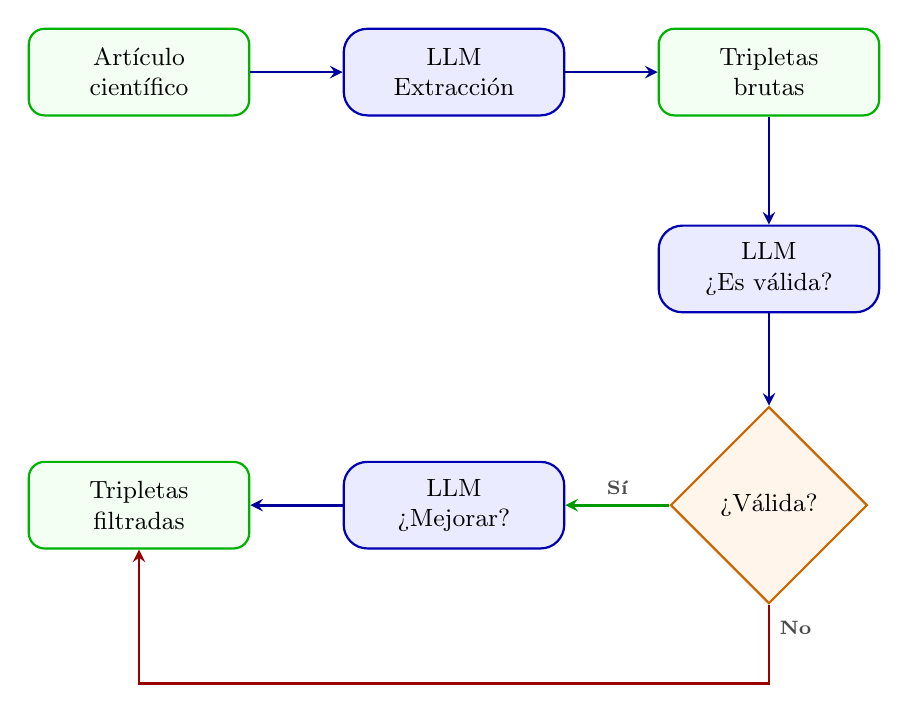
\begin{tikzpicture}[
    node distance=2.8cm and 3cm,
    every node/.style={align=center, font=\small},
    data/.style={rectangle, draw=green!70!black, fill=green!5, very thick, minimum width=2.8cm, minimum height=1.1cm, line width=0.8pt, rounded corners=2mm},
    process/.style={rectangle, rounded corners=3mm, draw=blue!70!black, fill=blue!8, very thick, minimum width=2.8cm, minimum height=1.1cm, line width=0.8pt},
    decision/.style={diamond, draw=orange!80!black, fill=orange!8, very thick, minimum width=2.5cm, minimum height=2.5cm, line width=0.8pt, aspect=1.5},
    arrow/.style={->, thick, >=stealth, line width=1pt},
    label/.style={font=\scriptsize\bfseries, text=black!70}
]

% --- Nodos principales
\node[data] (articulo) at (0,0) {Artículo\\científico};
\node[process] (llm1) at (4,0) {LLM\\Extracción};
\node[data] (tripletas1) at (8,0) {Tripletas\\brutas};

\node[process] (llm2) at (8,-2.5) {LLM\\¿Es válida?};
\node[decision] (decision) at (8,-5.5) {¿Válida?};

\node[process] (llm3) at (4,-5.5) {LLM\\¿Mejorar?};
\node[data] (tripletas_final) at (0,-5.5) {Tripletas\\filtradas};

% --- Flechas principales
\draw[arrow, blue!60!black] (articulo) -- (llm1);
\draw[arrow, blue!60!black] (llm1) -- (tripletas1);
\draw[arrow, blue!60!black] (tripletas1) -- (llm2);
\draw[arrow, blue!60!black] (llm2) -- (decision);

% Flecha Sí (decision -> llm3) - sale por la izquierda
\draw[arrow, green!60!black] (decision.west) -- node[label, above] {Sí} (llm3.east);

% Flecha No (decision -> tripletas_final) - sale por abajo
\draw[arrow, red!60!black] (decision.south) -- node[label, right, yshift=0.2cm] {No} ++(0,-1) -| (tripletas_final.south);

% Flecha final (llm3 -> tripletas_final)
\draw[arrow, blue!60!black] (llm3) -- (tripletas_final);

\end{tikzpicture}
\caption{Pipeline de doble filtrado LLM para extracción y validación de tripletas en artículos científicos.}
\label{fig:pipeline-articulos}
\end{figure}

\subsection{Ejemplos representativos}

\begin{itemize}
    \item Medicamentos:
    \begin{itemize}
        \item ⟨Abacavir, trata, infección por el virus de la inmunodeficiencia humana (VIH)⟩
        \item ⟨Niacina, dieta, seguir una dieta baja en grasa y colesterol⟩
        \item ⟨Crizotinib, efecto secundario, náuseas⟩
        \item ⟨Gilteritinib, almacenamiento, mantener en su empaque original, cerrado y fuera del alcance de los niños⟩
        \item ⟨Inyección de posaconazol, marca comercial, Noxafil⟩
        \item ⟨Inyección de pozelimab-bbfg, contraindicado en, infección meningocócica⟩
        \item ⟨Niraparib, se administra via, oral⟩
    \end{itemize}

    \item Pruebas de laboratorio:
    \begin{itemize}
        \item ⟨Densitometría ósea, mide, calcio y otros minerales en los huesos⟩
        \item ⟨Dióxido de carbono (CO2) en la sangre, requiere muestra de, sangre de una vena del brazo⟩
        \item ⟨Estudio del sueño, diagnostica, insomnio⟩
        \item ⟨Electroforesis de hemoglobina, tiene duracion, menos de cinco minutos⟩
        \item ⟨Examen de cáncer de piel, es tipo de, examen de detección⟩
        \item ⟨Examen dental, tiene riesgo, exposición a radiación baja⟩
    \end{itemize}

    \item Enfermedades:
    \begin{itemize}
        \item ⟨Hiperparatiroidismo, causada por, tumor hipersecretante⟩
        \item ⟨Alveolitis alérgica extrínseca, se diagnostica por, tumor leucocitosis⟩
        \item ⟨Hipertensión arterial, se asocia con, enfermedad coronaria⟩
        \item ⟨Hipertrigliceridemia, puede causar, infarto al miocardio⟩
        \item ⟨Hipocalcemia, se trata con, reposición de calcio por vía oral⟩
        \item ⟨Interrupción del arco aórtico, afecta órganos, arteria aorta⟩
        \item ⟨Malrotación intestinal, es congénita, sí⟩
        \item ⟨Aneurisma cerebral, nivel de gravedad, puede ser mortal⟩
        \item ⟨Colestasis del embarazo, afecta población, mujeres embarazadas⟩
    \end{itemize}

    \item Artículos científicos:
    \begin{itemize}
        \item ⟨anafilaxia, es un tipo de, reacción adversa de hipersensibilidad inmediata⟩
        \item ⟨Programa Nacional de Inmunizaciones (PNI), suministra, vacuna DPT (difteria, tos convulsiva y tétanos)⟩
        \item ⟨gafas plomadas, otorgan, protección contra radiación ionizante en órganos oculares⟩
        \item ⟨gafas plomadas, otorgan, protección contra radiación ionizante en órganos oculares⟩
        \item ⟨síndrome de Down, aumenta el riesgo de, malformaciones congénitas cardíacas⟩
        \item ⟨saliva, se utiliza para, la extracción de ADN genómico⟩
        \item ⟨encuesta poblacional en Chile, mide, daño a terceros producido por alcohol⟩
        \item ⟨cáncer gástrico, es la, primera causa de muerte por cáncer en Chile⟩
        \item ⟨población chilena, presenta, alta prevalencia de inactividad física⟩
        \item ⟨población mapuche, tiene, mayor prevalencia de cáncer de vesícula biliar⟩
        \item ⟨población aymara, tiene, bajo acceso a atención médica terciaria⟩
        \item ⟨ECLAMC, es un, programa de vigilancia epidemiológica de malformaciones congénitas en Latinoamérica⟩
        \item ⟨migrantes latinoamericanos, reportan, menor acceso y satisfacción con servicios de salud que chilenos⟩
    \end{itemize}
\end{itemize}

\begin{figure}[h]
\centering
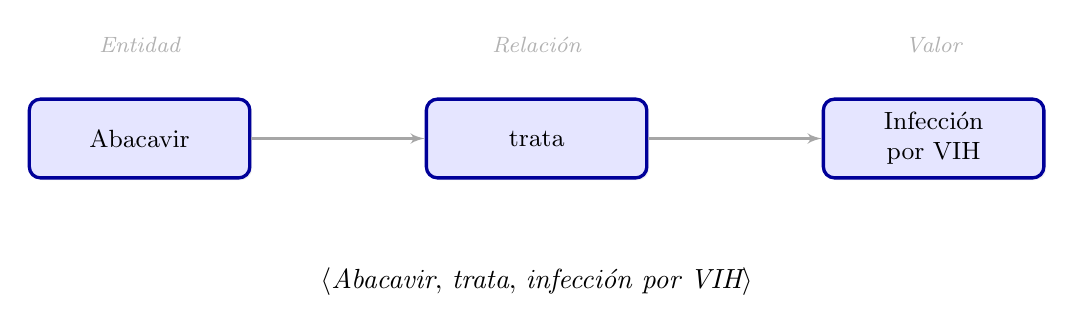
\begin{tikzpicture}[
    font=\small,
    box/.style={
        rectangle,
        rounded corners=4pt,
        draw=blue!60!black,
        fill=blue!10,
        minimum width=2.8cm,
        minimum height=1cm,
        very thick,
        align=center,
        drop shadow={shadow xshift=0.8pt, shadow yshift=-0.8pt, fill=gray!30, opacity=0.4}
    },
    arrow/.style={->, >=latex', thick, draw=gray!70},
    labelstyle/.style={font=\footnotesize\itshape, text=gray!60}
]

% --- Tripleta visual ---
\node[box] (entidad) {Abacavir};
\node[box, right=2.2cm of entidad] (relacion) {trata};
\node[box, right=2.2cm of relacion] (valor) {Infección\\por VIH};

% --- Flechas ---
\draw[arrow] (entidad) -- (relacion);
\draw[arrow] (relacion) -- (valor);

% --- Etiquetas superiores ---
\node[labelstyle, above=0.45cm of entidad] {Entidad};
\node[labelstyle, above=0.45cm of relacion] {Relación};
\node[labelstyle, above=0.45cm of valor] {Valor};

% --- Notación matemática inferior ---
\node[below=1cm of relacion, font=\normalsize] 
{$\langle \textit{Abacavir},\, \textit{trata},\, \textit{infección por VIH} \rangle$};

\end{tikzpicture}
\caption{Representación visual de una tripleta: relación entre entidad, relación y valor.}
\label{fig:ejemplo-tripleta}
\end{figure}


\begin{figure}[h]
\centering
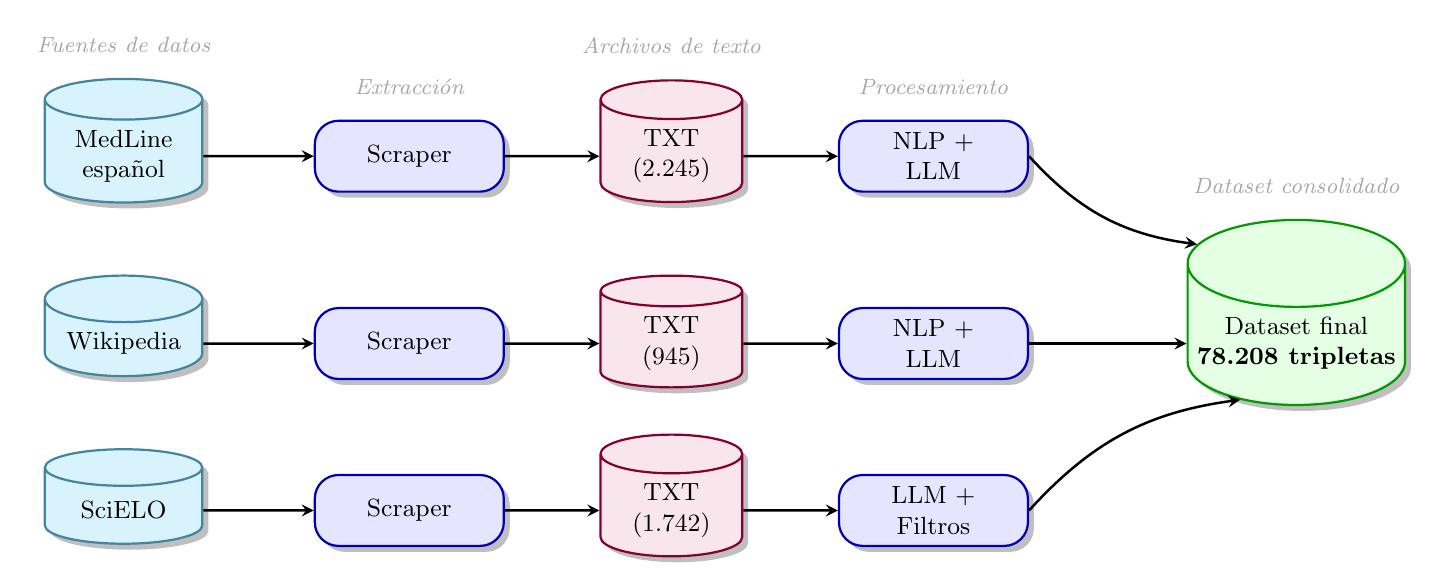
\begin{tikzpicture}[
    font=\small,
    node distance=1.6cm and 1.4cm,
    source/.style={cylinder, draw, shape border rotate=90, aspect=0.35, 
                   minimum height=1.2cm, minimum width=2cm,
                   fill=cyan!15, draw=cyan!60!black, thick, 
                   align=center, font=\small, drop shadow},
    process/.style={rectangle, draw, rounded corners=3mm, 
                    minimum width=2.4cm, minimum height=0.9cm,
                    align=center, fill=blue!10, draw=blue!70!black, thick, drop shadow},
    storage/.style={cylinder, draw, shape border rotate=90, aspect=0.4, 
                    minimum height=1cm, minimum width=1.8cm,
                    fill=purple!10, draw=purple!70!black, thick, align=center, drop shadow},
    arrow/.style={->, >=stealth, line width=0.9pt, rounded corners},
    label/.style={font=\footnotesize\itshape, gray!70}
]
% --- Fuentes de datos ---
\node[source] (medline) {MedLine\\español};
\node[source, below=0.9cm of medline] (wiki) {Wikipedia};
\node[source, below=0.9cm of wiki] (scielo) {SciELO};
% --- Scraping ---
\node[process, right=1.4cm of medline] (scrap1) {Scraper};
\node[process, right=1.4cm of wiki] (scrap2) {Scraper};
\node[process, right=1.4cm of scielo] (scrap3) {Scraper};
% --- Archivos de texto ---
\node[storage, right=1.2cm of scrap1] (txt1) {TXT\\(2.245)};
\node[storage, right=1.2cm of scrap2] (txt2) {TXT\\(945)};
\node[storage, right=1.2cm of scrap3] (txt3) {TXT\\(1.742)};
% --- Procesamiento ---
\node[process, right=1.2cm of txt1] (proc1) {NLP +\\LLM};
\node[process, right=1.2cm of txt2] (proc2) {NLP +\\LLM};
\node[process, right=1.2cm of txt3] (proc3) {LLM +\\Filtros};
% --- Dataset final ---
\node[storage, right=2cm of proc2, fill=green!10, draw=green!60!black] (dataset) 
    {Dataset final\\\textbf{78.208 tripletas}};
% --- Flechas ---
\foreach \a/\b in {medline/scrap1, wiki/scrap2, scielo/scrap3,
                   scrap1/txt1, scrap2/txt2, scrap3/txt3,
                   txt1/proc1, txt2/proc2, txt3/proc3}
    \draw[arrow] (\a) -- (\b);
\draw[arrow, bend right=20] (proc1.east) to (dataset.north west);
\draw[arrow] (proc2.east) -- (dataset.west);
\draw[arrow, bend left=20] (proc3.east) to (dataset.south west);
% --- Etiquetas visuales ---
\node[label, above=0.2cm of medline] {Fuentes de datos};
\node[label, above=0.2cm of scrap1] {Extracción};
\node[label, above=0.2cm of txt1] {Archivos de texto};
\node[label, above=0.2cm of proc1] {Procesamiento};
\node[label, above=0.2cm of dataset] {Dataset consolidado};
\end{tikzpicture}
\caption{Flujo completo desde las fuentes hasta la consolidación del dataset final.}
\label{fig:flujo-completo}
\end{figure}

\subsection{Análisis de fortalezas y debilidades}

Los datasets son muy robustos, siendo en su gran mayoría tripletas relevantes como se observan en los ejemplos. Para los medicamentos, pruebas de laboratorio y enfermedades, la estructura de los documentos originales facilitó sustancialmente la creación de la tripletas y esto llevó a muy buenos resultados. En el caso de los artículos científicos, hubo un mayor desafío.

Haciendo una revisión manual, las tripletas de los medicamentos y las enfermedades son prácticamente perfectas: no se encontró algún ejemplo de debilidad relevante. En el caso de las pruebas médicas se encontraron algunas debilidades. Por ejemplo, ⟨Evaluación de depresión, alivia, síntomas de depresión⟩ donde esta prueba, al ser una evaluación, no alivia los síntomas, si no que podría ayudar a comenzar a aliviar los síntomas. Otro ejemplo es ⟨Nefritis intersticial aguda, presenta síntoma, leucocitos⟩, donde falta contexto en el valor. Es decir, qué ocurre con los leucocitos: si disminuye el conteo, aumenta u otro tipo de variación.

Sobre los artículos científicos, al realizar el filtro estos mejoraron sustancialmente. Se eliminaron muchas tripletas a las que le faltaba contexto y de cosas específicas del artículo. De todas formas, hay algunas tripletas que se mantuvieron como por ejemplo ⟨edad media al diagnóstico, es, 56,77 años⟩, donde falta saber qué diagnósticos. Otro ejemplo es ⟨hijos de madres entre 20 y 34 años, tienen, tasa de malformaciones congénitas⟩ al que le falta contexto. Otro tipo de caso es ⟨dosis equivalente máxima, sugiere, 20 mSv/año para el cristalino⟩, donde el valor tiene parte de la entidad (cristalino). Por último, se detectó un caso donde la entidad no es una entidad: ⟨igual, igual, métodos estadísticos como Kaplan-Meier y análisis multivariante con modelo de riesgos proporcionales de Cox⟩.

A pesar de las pocas debilidades, la parte de los artículos científicos es muy relevante. Existen muchos datos que son específicos a Latinoamérica y Chile. Por ejemplo, hay más de 300 tripletas que hacen referencia a Chile o chilenos. Así mismo, hay ejemplos específicos de etnias indígenas como los mostrados anteriormente de la población mapuche y aymara.

\section{Informe de evaluación}

\subsection{Procedimiento de la evaluación}

Para la evaluación de los modelos se realizó un script que cree preguntas, luego genere las respuestas por modelo y por último la evaluación de las respuestas. Para todo este procedimiento se ocupó OpenRouter \cite{openrouter}, variando los prompts y los modelos usados. Primero, para generar las preguntas de los medicamentos, pruebas de laboratorio y enfermedades, se generaron a partir de las relaciones recomendadas. En el caso de los medicamentos y las pruebas de laboratorio, el mismo texto original tenía preguntas como por ejemplo "¿Para cuáles condiciones o enfermedades se prescribe este $<$medicamento$>$?" Es importante mencionar que para una misma pregunta, pueden haber varias tripletas asociadas y por ende, las respuestas deberían tener todos esos valores (ver Figura \ref{fig:ejemplo-multiples-valores}). Adicionalmente se agregaron otras preguntas según la relación. Por ejemplo, para la relación "se administra vía" se creó la pregunta "¿Por qué vía se administra $<$medicamento$>$?" En el caso de las enfermedades se siguió la misma técnica al crear las preguntas. Por ejemplo, para la relación "se trata con" se creó la pregunta "¿Cuáles son los tratamientos o intervenciones de la enfermedad/condición $<$enfermedad$>$?"

\begin{figure}[h]
\centering
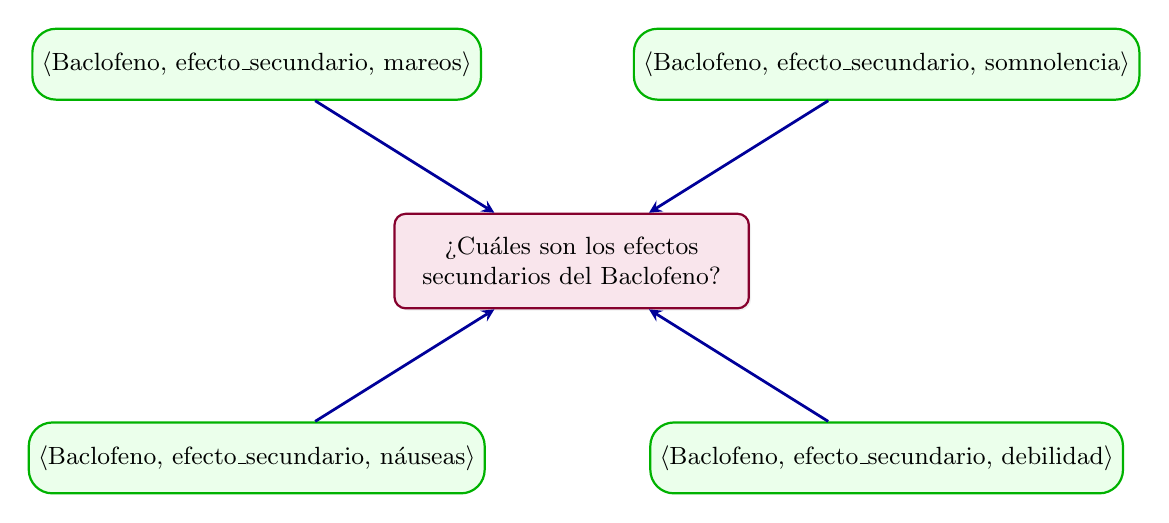
\begin{tikzpicture}[
    font=\small,
    question/.style={
        rectangle,
        rounded corners=4pt,
        draw=purple!70!black,
        fill=purple!10,
        minimum width=4.5cm,
        minimum height=1.2cm,
        very thick,
        align=center,
        line width=0.8pt,
        drop shadow={shadow xshift=0.8pt, shadow yshift=-0.8pt, fill=gray!30, opacity=0.4}
    },
    triplet/.style={
        rectangle,
        rounded corners=3mm,
        draw=green!70!black,
        fill=green!8,
        minimum width=5.5cm,
        minimum height=0.9cm,
        very thick,
        align=center,
        line width=0.8pt,
        font=\small
    },
    arrow/.style={->, >=stealth, thick, line width=1pt, draw=blue!60!black},
    labelstyle/.style={font=\scriptsize\itshape, text=gray!60}
]

% Pregunta (centro)
\node[question] (pregunta) at (0,0) {¿Cuáles son los efectos\\secundarios del Baclofeno?};

% Tripletas alrededor
\node[triplet] (t1) at (-4,2.5) {$\langle$Baclofeno, efecto\_secundario, mareos$\rangle$};
\node[triplet] (t2) at (4,2.5) {$\langle$Baclofeno, efecto\_secundario, somnolencia$\rangle$};
\node[triplet] (t3) at (-4,-2.5) {$\langle$Baclofeno, efecto\_secundario, náuseas$\rangle$};
\node[triplet] (t4) at (4,-2.5) {$\langle$Baclofeno, efecto\_secundario, debilidad$\rangle$};

% Flechas apuntando hacia la pregunta desde cada esquina
\draw[arrow] (t1) -- (pregunta);
\draw[arrow] (t2) -- (pregunta);
\draw[arrow] (t3) -- (pregunta);
\draw[arrow] (t4) -- (pregunta);


\end{tikzpicture}
\caption{Representación visual de una pregunta con varios valores de tripletas asociadas.}
\label{fig:ejemplo-multiples-valores}
\end{figure}

En el caso de los artículos científicos, dado que se crearon las tripletas sin entregar la entidad ni recomendar las relaciones, se creó una pregunta por cada tripleta. Para esto, se ocupó un LLM (\texttt{gpt-4o-mini}) para que cree las preguntas, considerando la información de la tripleta. Por ejemplo, para la tripleta ⟨Chile, es un, país con alta mortalidad por cáncer gástrico⟩ se creó la pregunta "¿Cómo se caracteriza Chile respecto a la mortalidad por cáncer gástrico?" o para la tripleta ⟨Entrevista de Acceso Privilegiado (EAP), es una, metodología cualitativa para estudiar poblaciones ocultas⟩ la pregunta "¿Qué tipo de metodología es la Entrevista de Acceso Privilegiado (EAP)?"

Una vez se generaron todas las preguntas, se procedió a generar las respuestas para cada modelo: Qwen 2.5 7B, Llama 3.1 8B y Mistral 0.3 7B. Para esto, se le pidió a cada modelo responder todas las preguntas, almacenando esta información. Luego, ocupando (\texttt{gpt-4o-mini}) se evaluó cada respuesta de forma binaria con "correcto" o "incorrecto", comparando con los valores de la tripleta original. Una representación visual del procedimiento de la evaluación se puede apreciar en la Figura \ref{fig:pipeline-evaluacion}.

\begin{figure}[h]
\centering
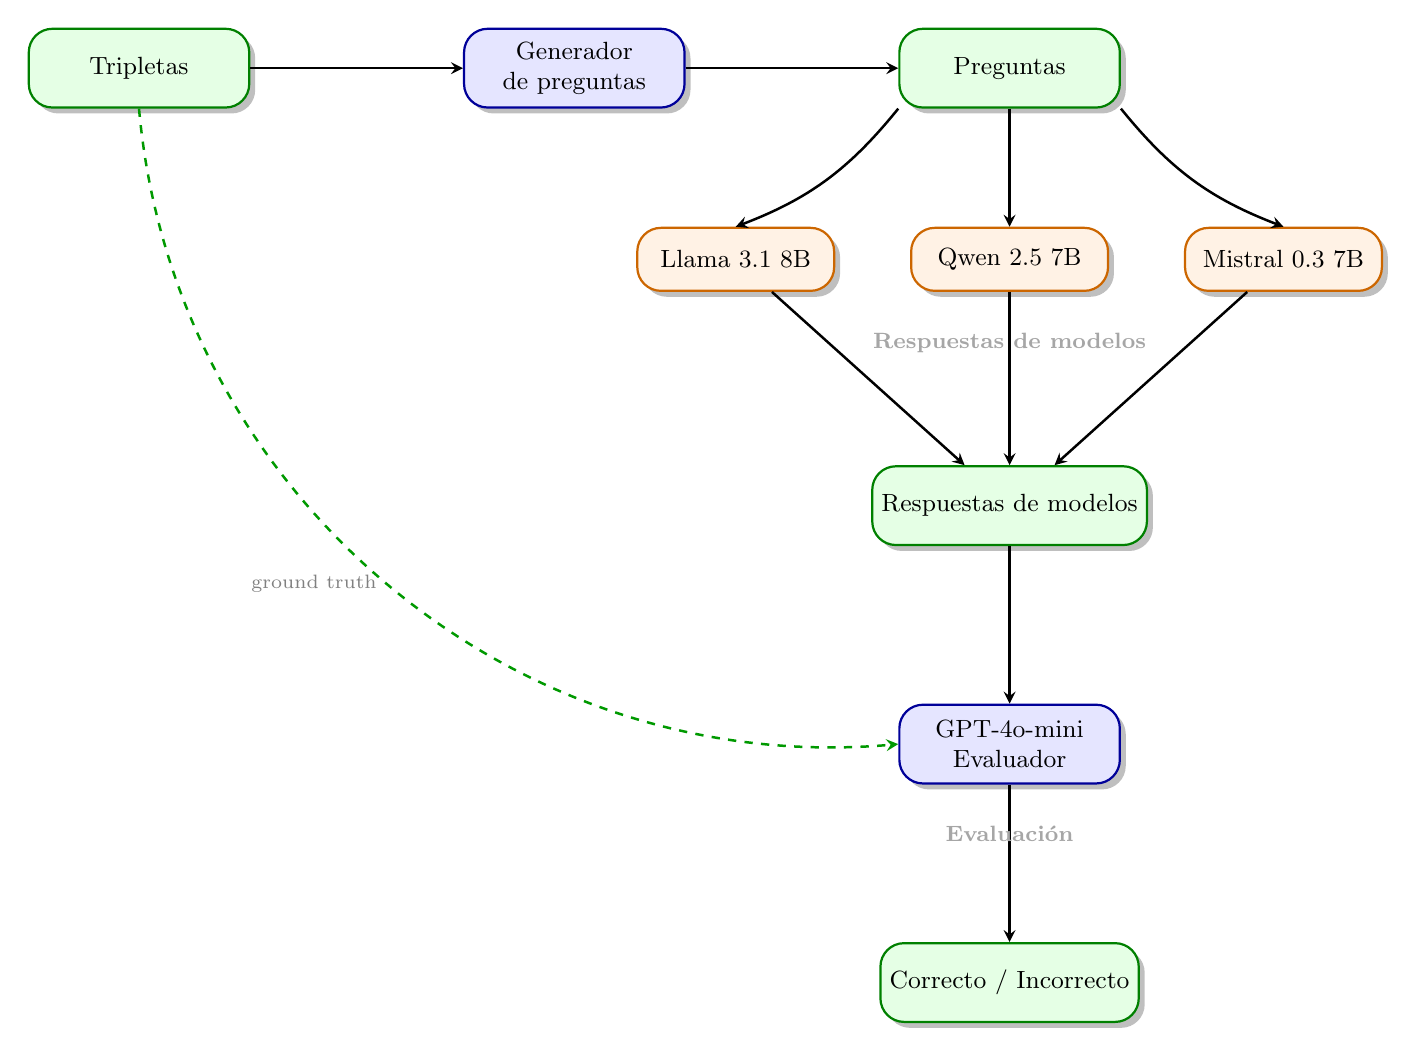
\begin{tikzpicture}[
    font=\small,
    node distance=2.3cm and 2.7cm,
    data/.style={rectangle, rounded corners=3mm, draw=green!50!black, fill=green!10, thick,
                 minimum width=2.8cm, minimum height=1cm, align=center, drop shadow},
    process/.style={rectangle, rounded corners=3mm, draw=blue!60!black, fill=blue!10, thick,
                    minimum width=2.8cm, minimum height=1cm, align=center, drop shadow},
    model/.style={rectangle, rounded corners=3mm, draw=orange!80!black, fill=orange!10, thick,
                  minimum width=2.5cm, minimum height=0.8cm, align=center, drop shadow},
    arrow/.style={->, >=stealth, line width=0.9pt, rounded corners},
    every label/.style={font=\footnotesize\itshape, gray!70}
]

% --- Etapa 1: Generación de preguntas ---
\node[data] (tripletas) {Tripletas};
\node[process, right=of tripletas] (gen_preg) {Generador\\de preguntas};
\node[data, right=of gen_preg] (preguntas) {Preguntas};

% --- Etapa 2: Modelos responden ---
\node[model, below left=1.5cm and 0.8cm of preguntas] (llama) {Llama 3.1 8B};
\node[model, below=1.5cm of preguntas] (qwen) {Qwen 2.5 7B};
\node[model, below right=1.5cm and 0.8cm of preguntas] (mistral) {Mistral 0.3 7B};
\node[data, below=2.2cm of qwen] (respuestas) {Respuestas de modelos};

% --- Etapa 3: Evaluación ---
\node[process, below=2.0cm of respuestas] (evaluador) {GPT-4o-mini\\Evaluador};
\node[data, below=2.0cm of evaluador] (resultados) {Correcto / Incorrecto};

% --- Flechas ---
\draw[arrow] (tripletas) -- (gen_preg);
\draw[arrow] (gen_preg) -- (preguntas);

\draw[arrow, bend left=15] (preguntas.south west) to (llama.north);
\draw[arrow] (preguntas) -- (qwen);
\draw[arrow, bend right=15] (preguntas.south east) to (mistral.north);

\draw[arrow] (llama) -- (respuestas);
\draw[arrow] (qwen) -- (respuestas);
\draw[arrow] (mistral) -- (respuestas);

\draw[arrow] (respuestas) -- (evaluador);

% Flecha punteada desde el centro
\draw[arrow, bend right=45, dashed, green!60!black]
    (tripletas.south) to node[midway, left, font=\scriptsize, gray]{ground truth} (evaluador.west);

\draw[arrow] (evaluador) -- (resultados);

% --- Títulos visuales ---
\node[below=0.4cm of qwen, font=\footnotesize\bfseries, gray!70]{Respuestas de modelos};
\node[below=0.4cm of evaluador, font=\footnotesize\bfseries, gray!70]{Evaluación};

\end{tikzpicture}
\caption{Pipeline completo de evaluación de modelos.}
\label{fig:pipeline-evaluacion}
\end{figure}

\subsection{Ejemplos representativos}

\begin{itemize}
    \item Qwen 2.5 7B:
    \begin{itemize}
        \item Tripleta: ⟨Abrocitinib, marca comercial, Cibinqo ®⟩
        \begin{itemize}
            \item Pregunta: ¿Cuáles son las marcas comerciales de Abrocitinib?
            \item Respuesta: The brand name for Abrocitinib is Cimzia. However, there seems to be a misunderstanding as Abrocitinib is actually marketed under the brand name Rinvoq by Pfizer.
            \item Evaluación: incorrecto
        \end{itemize}

        \item Tripleta: ⟨Simeticona, olvido, tomar la dosis olvidada tan pronto como lo recuerde, omitir si es casi hora de la siguiente dosis⟩
        \begin{itemize}
            \item Pregunta: ¿Qué tengo que hacer si me olvido de tomar una dosis de Simeticona?
            \item Respuesta: Si te olvidas de tomar una dosis de Simeticona, toma la dosis olvidada lo antes posible. Si es cerca de la hora de tu dosis siguiente, ignora la dosis olvidada y toma la siguiente dosis a su hora programada. No dobles la dosis. Si estás usando Simeticona regularmente para una condición persistente, consulta a tu médico si un olvido en la dosis es preocupante.
            \item Evaluación: correcto
        \end{itemize}

        \item Tripleta: ⟨Densitometría ósea, tiene duración, entre 10 y 30 minutos⟩
        \begin{itemize}
            \item Pregunta: ¿Cuánto dura Densitometría ósea?
            \item Respuesta: El tiempo de duración de una densitometría ósea varía dependiendo del método utilizado, pero generalmente dura entre 5 y 30 minutos.
            \item Evaluación: correcto
        \end{itemize}
        
        \item Tripleta: ⟨Diarrea, se asocia con, reducción del consumo de alimento⟩
        \begin{itemize}
            \item Pregunta: ¿Con qué otras condiciones médicas se relaciona la enfermedad/condición Diarrea?
            \item Respuesta: La diarrea puede $<$símbolos en chino$>$.
            \item Evaluación: incorrecto
        \end{itemize}

        \item Tripleta: ⟨deterioro cognitivo, afecta, cerca de 200.000 personas en Chile⟩
        \begin{itemize}
            \item Pregunta: ¿Cuántas personas en Chile afectan el deterioro cognitivo?
            \item Respuesta: No hay datos específicos disponibles sobre el número exacto de personas en Chile que afectan directamente el deterioro cognitivo. El deterioro cognitivo es...
            \item Evaluación: incorrecto
        \end{itemize}
    \end{itemize}

    \item Llama 3.1 8B:
    \begin{itemize}
        \item Tripleta: ⟨terconazol, almacenamiento, mantener en su envase, bien cerrado y fuera del alcance de los niños, guardar a temperatura ambiente y lejos del calor y la humedad⟩
        \begin{itemize}
            \item Pregunta: ¿Cómo debo almacenar terconazol?
            \item Respuesta: En un lugar fresco y seco, alejado de la luz directa del sol, protegido de niños y animales.
            \item Evaluación: correcto
        \end{itemize}
        
        \item Tripleta: ⟨Prueba de Papanicolaou, utiliza equipo, espéculo⟩
        \begin{itemize}
            \item Pregunta: ¿Qué equipo utiliza Prueba de Papanicolaou?
            \item Respuesta: La prueba de Papanicolaou requiere el uso de un microscopio o ungetitem afluoroscopio.
            \item Evaluación: incorrecto
        \end{itemize}
        
        \item Tripleta: ⟨Rotura del timpano, afecta organos, oído⟩
        \begin{itemize}
            \item Pregunta: ¿Qué órganos o sistemas son afectados por la enfermedad/condición Rotura del timpano?
            \item Respuesta: El sistema auditivo.
            \item Evaluación: correcto
        \end{itemize}
        
        \item Tripleta: ⟨score de Blatchford, se utiliza para, evaluar riesgo de necesitar intervención clínica en hemorragia digestiva alta⟩
        \begin{itemize}
            \item Pregunta: ¿Para qué se utiliza el score de Blatchford?
            \item Respuesta: Para evaluar la complejidad de los procesos judiciales.
            \item Evaluación: incorrecto
        \end{itemize}
    \end{itemize}
    
    \item Mistral 0.3 7B:
    \begin{itemize}
        \item Tripleta: ⟨Isocarboxazida, trata, depresión en personas donde otros antidepresivos no han dado resultado⟩
        \begin{itemize}
            \item Pregunta: ¿Para cuáles condiciones o enfermedades se prescribe Isocarboxazida?
            \item Respuesta: Isocarboxazida se prescribe principalmente para el tratamiento de la enfermedad de Parkinson.
            \item Evaluación: incorrecto
        \end{itemize}
    
        \item Tripleta: ⟨Pruebas de Helicobacter pylori, realizado por, profesional de la salud⟩
        \begin{itemize}
            \item Pregunta: ¿Quién realiza Pruebas de Helicobacter pylori?
            \item Respuesta: Un gastroenterólogo o un médico especializado en enfermedades del aparato digestivo.
            \item Evaluación: correcto
        \end{itemize}
        
        \item Tripleta: ⟨Enfermedad poliquística renal, es hereditaria, sí⟩
        \begin{itemize}
            \item Pregunta: ¿Es la enfermedad/condición Enfermedad poliquística renal hereditaria o no?
            \item Respuesta: Sí, la enfermedad poliquística renal es hereditaria.
            \item Evaluación: correcto
        \end{itemize}
        
        \item Tripleta: ⟨ECLAMC, es un, programa de vigilancia epidemiológica de malformaciones congénitas en Latinoamérica⟩
        \begin{itemize}
            \item Pregunta: ¿Qué tipo de programa es el ECLAMC?
            \item Respuesta: El ECLAMC es un programa de computación.
            \item Evaluación: incorrecto
        \end{itemize}
    \end{itemize}
\end{itemize}

\subsection{Descripción general de la evaluación}

La evaluación de los tres modelos de lenguaje se realizó sobre un conjunto de 131.088 instancias distribuidas en cuatro categorías del dominio de la salud. La distribución de las evaluaciones refleja la estructura del dataset construido, donde los medicamentos constituyen la categoría más voluminosa con 55.782 evaluaciones (42,6\% del total), seguida por los artículos científicos con 46.032 evaluaciones (35,1\%). Las enfermedades representan 21.027 evaluaciones (16,0\%), mientras que los exámenes de laboratorio, siendo la categoría más pequeña, contienen 8.247 evaluaciones (6,3\% del total). Esta distribución proporciona una base robusta para analizar el desempeño de los modelos en diferentes tipos de conocimiento médico, desde información estructurada sobre medicamentos hasta conocimiento más contextual presente en artículos científicos latinoamericanos.

\subsection{Resultados cuantitativos}

La Tabla~\ref{tab:resultados_detallados} presenta los resultados completos de la evaluación, incluyendo tanto las frecuencias absolutas como los porcentajes de precisión para cada modelo en las distintas categorías. Los resultados revelan diferencias sustanciales en el desempeño de los tres modelos evaluados, con rangos de precisión que varían desde el 12,00\% hasta el 53,94\% dependiendo del modelo y la categoría considerada.

\begin{table}[htbp]
\centering
\caption{Resultados detallados de evaluación por modelo y categoría}
\label{tab:resultados_detallados}
\resizebox{\textwidth}{!} & \textbf{C} & \textbf{I} & \textbf{\%} & \textbf{C} & \textbf{I} & \textbf{\%} & \textbf{C} & \textbf{I} & \textbf{\%} & \textbf{C} & \textbf{I} & \textbf{\%} \\
\hline
Qwen 2.5 7B & 8.139 & 10.455 & 43,77 & 3.129 & 3.880 & 44,64 & 1.006 & 1.443 & 41,09 & 4.624 & 10.720 & 30,14 & 16.898 & 26.498 & \textbf{38,94} \\
Llama 3.1 8B & 2.231 & 16.363 & 12,00 & 2.110 & 4.899 & 30,10 & 1.002 & 1.947 & 33,98 & 2.731 & 12.613 & 17,80 & 8.074 & 35.822 & \textbf{18,39} \\
Mistral 0.3 7B & 7.440 & 11.154 & 40,01 & 3.781 & 3.228 & 53,94 & 1.418 & 1.431 & 49,77 & 4.843 & 10.501 & 31,56 & 17.482 & 26.314 & \textbf{39,92} \\
\hline
\textbf{Total} & \multicolumn{2}{c}{55.782} & & \multicolumn{2}{c}{21.027} & & \multicolumn{2}{c}{8.247} & & \multicolumn{2}{c}{46.032} & & \multicolumn{2}{c}{131.088} & \\
\hline
\end{tabular}%
}

\vspace{2mm}
\small
C = Correctas; I = Incorrectas; \% = Porcentaje de precisión
\end{table}

El análisis global de desempeño muestra que Mistral 0.3 7B alcanza la mayor precisión con un 39,92\% de respuestas correctas, superando marginalmente a Qwen 2.5 7B que obtiene un 38,94\%. En contraste, Llama 3.1 8B presenta un desempeño significativamente inferior con apenas un 18,39\% de precisión, lo que representa menos de la mitad del rendimiento de los otros dos modelos. Esta brecha tan marcada sugiere diferencias fundamentales en la arquitectura, datos de entrenamiento, o ambos factores, especialmente en lo que respecta a contenido médico en español.

\subsection{Análisis estadístico inferencial}

Para determinar si las diferencias observadas entre modelos son estadísticamente significativas, se realizó un test de proporciones Z para cada par de modelos comparando su desempeño global. Los resultados confirmaron que las diferencias son altamente significativas en todos los casos. La comparación entre Qwen y Llama arrojó un Z-score de 67,16 ($p < 0,001$), mientras que la comparación entre Mistral y Llama produjo un Z-score de 70,13 ($p < 0,001$). Incluso la diferencia aparentemente pequeña entre Qwen y Mistral resultó ser estadísticamente significativa con un Z-score de -2,95 ($p = 0,003$), favoreciendo a Mistral. Estos resultados indican que las diferencias observadas no son producto del azar, sino que reflejan diferencias reales en la capacidad de los modelos para responder correctamente preguntas sobre contenido médico en español.

Adicionalmente, se aplicó un test de independencia chi-cuadrado para evaluar si existe una relación entre el tipo de modelo y su desempeño en las diferentes categorías. El estadístico chi-cuadrado obtenido fue de 1.075,56 con 6 grados de libertad ($p < 0,001$), lo que indica una dependencia significativa entre el modelo y la categoría. Este resultado sugiere que los modelos no solo difieren en su desempeño global, sino que además presentan perfiles de fortalezas y debilidades específicos para cada tipo de contenido médico.

\subsection{Análisis por categoría}

La Tabla~\ref{tab:estadisticas_categoria} resume las estadísticas descriptivas para cada categoría, revelando patrones importantes en el desempeño de los modelos según el tipo de contenido evaluado.

\begin{table}[htbp]
\centering
\caption{Estadísticas descriptivas por categoría}
\label{tab:estadisticas_categoria}
\begin{tabular}{lrrrr}
\hline
\textbf{Categoría} & \textbf{n} & \textbf{Media (\%)} & \textbf{DE} & \textbf{Rango (\%)} \\
\hline
Medicamentos & 55.782 & 31,93 & 17,36 & 12,00 -- 43,77 \\
Enfermedades & 21.027 & 42,89 & 12,02 & 30,10 -- 53,94 \\
Exámenes & 8.247 & 41,61 & 7,91 & 33,98 -- 49,77 \\
Artículos & 46.032 & 26,50 & 7,57 & 17,80 -- 31,56 \\
\hline
\end{tabular}

\vspace{2mm}
\small
n = número de evaluaciones; DE = desviación estándar
\end{table}

\subsubsection{Medicamentos}

La categoría de medicamentos, con 55.782 evaluaciones, presenta la mayor dispersión en el desempeño entre modelos, evidenciada por una desviación estándar de 17,36 puntos porcentuales y un rango de 31,77 puntos entre el mejor y peor modelo. Qwen 2.5 7B lidera esta categoría con una precisión del 43,77\%, logrando clasificar correctamente 8.139 de las 18.594 preguntas evaluadas. Este rendimiento superior sugiere que el modelo ha sido expuesto a una cantidad sustancial de literatura farmacológica durante su entrenamiento. Mistral 0.3 7B, con un 40,01\% de precisión, se mantiene competitivo aunque ligeramente por debajo de Qwen. Sin embargo, Llama 3.1 8B colapsa en esta categoría con apenas un 12,00\% de precisión, acertando solamente 2.231 de 18.594 preguntas. Esta diferencia tan marcada indica que Llama tiene una representación deficiente del conocimiento farmacológico en español, posiblemente debido a un desbalance en sus datos de entrenamiento que favoreció otros dominios o idiomas.

\subsubsection{Enfermedades}

En el dominio de enfermedades, que comprende 21.027 evaluaciones, los modelos muestran su mejor desempeño promedio con un 42,89\% de precisión. Mistral 0.3 7B sobresale significativamente con una precisión del 53,94\%, respondiendo correctamente 3.781 de 7.009 preguntas. Este es el porcentaje más alto alcanzado por cualquier modelo en cualquier categoría, sugiriendo que Mistral ha desarrollado una representación particularmente robusta del conocimiento sobre enfermedades. Qwen 2.5 7B obtiene un desempeño respetable del 44,64\%, mientras que Llama 3.1 8B mejora considerablemente respecto a su desempeño en medicamentos, alcanzando un 30,10\%. La menor dispersión entre modelos en esta categoría, reflejada en una desviación estándar de 12,02 puntos, sugiere que la información sobre enfermedades está más uniformemente representada en los corpus de entrenamiento de los distintos modelos, aunque con diferencias cuantitativas importantes.

\subsubsection{Exámenes de laboratorio}

La categoría de exámenes de laboratorio, siendo la más pequeña con 8.247 evaluaciones, presenta características interesantes. Mistral 0.3 7B lidera nuevamente con una precisión del 49,77\%, clasificando correctamente 1.418 de 2.849 preguntas. El aspecto más notable de esta categoría es la convergencia relativa del desempeño entre Qwen (41,09\%) y Llama (33,98\%), evidenciada por la menor desviación estándar entre categorías (7,91 puntos). Esta convergencia sugiere que el conocimiento sobre procedimientos diagnósticos básicos está más uniformemente distribuido entre los modelos. El rango de solo 15,79 puntos porcentuales entre el mejor y peor modelo contrasta marcadamente con los 31,77 puntos observados en medicamentos, indicando que esta categoría representa un desafío más homogéneo para los modelos evaluados.

\subsubsection{Artículos científicos}

Los artículos científicos latinoamericanos constituyen el mayor desafío para todos los modelos, presentando el desempeño promedio más bajo con apenas un 26,50\% de precisión. Mistral 0.3 7B alcanza un 31,56\% de precisión con 4.843 respuestas correctas de 15.344 evaluaciones, seguido por Qwen 2.5 7B con un 30,14\%. Llama 3.1 8B, consistente con su patrón de bajo desempeño, obtiene solo un 17,80\% de precisión. La dificultad generalizada en esta categoría es particularmente reveladora del problema central que motiva este trabajo: la subrepresentación del conocimiento latinoamericano en los modelos de lenguaje de frontera. Los artículos contienen información específica sobre prevalencias de enfermedades en poblaciones chilenas, características epidemiológicas de comunidades indígenas (mapuche, aymara), y contextos de salud pública locales que evidentemente no están bien representados en los datos de entrenamiento de ninguno de los modelos evaluados. Esta categoría expone una limitación sistemática que trasciende las diferencias arquitectónicas o de tamaño entre los modelos.

\subsection{Variabilidad de desempeño intra-modelo}

El análisis de la variabilidad de desempeño de cada modelo a través de las categorías proporciona información adicional sobre su consistencia. La Tabla~\ref{tab:variabilidad} presenta métricas de dispersión para cada modelo.

\begin{table}[htbp]
\centering
\caption{Variabilidad de desempeño por modelo}
\label{tab:variabilidad}
\begin{tabular}{lrrrr}
\hline
\textbf{Modelo} & \textbf{Media (\%)} & \textbf{DE} & \textbf{CV (\%)} & \textbf{Rango (\%)} \\
\hline
Qwen 2.5 7B & 39,91 & 5,79 & 14,51 & 14,50 \\
Llama 3.1 8B & 23,47 & 8,92 & 38,00 & 21,98 \\
Mistral 0.3 7B & 43,82 & 8,70 & 19,85 & 22,38 \\
\hline
\end{tabular}

\vspace{2mm}
\small
DE = desviación estándar; CV = coeficiente de variación
\end{table}

Qwen 2.5 7B exhibe la mayor consistencia entre categorías con un coeficiente de variación del 14,51\% y un rango de solo 14,50 puntos porcentuales entre su mejor (44,64\% en enfermedades) y peor (30,14\% en artículos) categoría. Esta consistencia sugiere un modelo bien balanceado que mantiene un nivel de desempeño relativamente estable independientemente del tipo de contenido médico. En contraste, Llama 3.1 8B presenta la mayor variabilidad con un coeficiente de variación del 38,00\% y un rango de 21,98 puntos porcentuales. Esta alta variabilidad, combinada con su bajo desempeño promedio del 23,47\%, indica no solo un rendimiento global deficiente sino también una representación desigual del conocimiento médico a través de diferentes dominios. Mistral 0.3 7B, a pesar de tener el mejor desempeño promedio (43,82\%), presenta una variabilidad intermedia con un coeficiente de variación del 19,85\%, reflejando fortalezas particulares en enfermedades y exámenes, pero debilidades relativas en artículos científicos.

\subsection{Análisis cualitativo de respuestas}

El análisis cualitativo de las respuestas generadas complementa los hallazgos cuantitativos y revela patrones específicos de error y acierto. En el caso de Qwen 2.5 7B, se observó que el modelo puede generar respuestas incorrectas con alta confianza aparente. Por ejemplo, ante la pregunta sobre las marcas comerciales de Abrocitinib, el modelo respondió inicialmente mencionando "Cimzia" y luego corrigió a "Rinvoq by Pfizer", cuando la marca correcta es "Cibinqo". Este tipo de error, donde el modelo confunde marcas comerciales de diferentes medicamentos, sugiere que aunque el modelo tiene conocimiento farmacológico sustancial, ocasionalmente confunde entidades similares o relacionadas.

Por otro lado, cuando Qwen 2.5 7B responde correctamente, sus respuestas muestran una estructura coherente y completa. Ante la pregunta sobre qué hacer si se olvida una dosis de Simeticona, el modelo generó una respuesta que capturaba correctamente la información de la tripleta (tomar la dosis olvidada tan pronto como se recuerde, omitir si es casi hora de la siguiente) y además agregó información contextual relevante como la advertencia de no duplicar la dosis y la recomendación de consultar al médico si hay preocupación. Esta capacidad de expandir apropiadamente sobre la información básica, manteniendo la precisión factual, representa una fortaleza del modelo.

Los errores de Llama 3.1 8B tienden a ser más fundamentales, frecuentemente confundiendo conceptos básicos o proporcionando información genérica que no responde específicamente a la pregunta planteada. Esto es consistente con su bajo desempeño cuantitativo y sugiere una limitación más profunda en su conocimiento del dominio médico en español. Mistral 0.3 7B, cuando genera respuestas correctas, tiende a ser conciso pero preciso, aunque ocasionalmente omite detalles contextuales que podrían enriquecer la respuesta.

\subsection{Implicaciones del conocimiento regional}

Un hallazgo particularmente significativo emerge del análisis del desempeño en artículos científicos, que constituyen la única categoría con información predominantemente regional. El dataset incluye más de 300 tripletas que hacen referencia explícita a Chile, poblaciones chilenas, o comunidades indígenas específicas como los mapuche y aymara. El bajo desempeño generalizado en esta categoría (ningún modelo supera el 31,56\% de precisión) contrasta marcadamente con el rendimiento en categorías de conocimiento médico más universal como enfermedades (hasta 53,94\%) o exámenes (hasta 49,77\%).

Esta brecha de aproximadamente 20 puntos porcentuales entre el conocimiento universal y el regional no puede atribuirse únicamente a diferencias en la complejidad de las preguntas, ya que tanto las tripletas de enfermedades como las de artículos científicos involucran relaciones complejas entre múltiples conceptos. En cambio, el patrón sugiere fuertemente que los modelos evaluados han tenido exposición limitada o nula a literatura científica latinoamericana durante su entrenamiento. Considerando que el dataset contiene información como la prevalencia específica de cáncer gástrico en Chile, las tasas de malformaciones congénitas en diferentes grupos etarios chilenos, o las características de acceso a atención médica en poblaciones indígenas, la incapacidad de los modelos para capturar este conocimiento representa una limitación significativa para su aplicabilidad en contextos de salud pública latinoamericanos.

\subsection{Relación entre debilidades del dataset y desempeño}

El análisis de los resultados también permite identificar cómo ciertas debilidades documentadas del dataset impactan la evaluación. Las tripletas con contexto insuficiente, particularmente prevalentes en la categoría de exámenes médicos, probablemente contribuyen a respuestas que son evaluadas como incorrectas incluso cuando el modelo ha captado la esencia correcta de la información. Por ejemplo, la tripleta problemática identificada ⟨Nefritis intersticial aguda, presenta síntoma, leucocitos⟩ carece de especificación sobre qué ocurre con los leucocitos (incremento, disminución, presencia en orina), lo que dificulta tanto para el modelo como para el evaluador determinar qué constituye una respuesta correcta.

En el caso de los artículos científicos, algunas tripletas retuvieron información demasiado específica del artículo original sin contexto adecuado, como ⟨edad media al diagnóstico, es, 56,77 años⟩ donde falta especificar el diagnóstico en cuestión. Estas ambigüedades introducen ruido en la evaluación, aunque su impacto es limitado dado que representan una fracción minoritaria del dataset total de 78.208 tripletas. Las tripletas problemáticas identificadas en las pruebas de laboratorio y artículos científicos representan menos del 2\% del total, por lo que su influencia en las conclusiones generales es marginal.

\subsection{Síntesis de hallazgos}

Los resultados de esta evaluación revelan tres hallazgos principales. Primero, existe una jerarquía clara de desempeño entre los modelos evaluados, con Mistral 0.3 7B y Qwen 2.5 7B demostrando capacidades significativamente superiores a Llama 3.1 8B para procesar y responder preguntas sobre contenido médico en español. Las diferencias son estadísticamente significativas y consistentes a través de todas las categorías evaluadas. Segundo, el desempeño de los modelos varía sustancialmente según el tipo de contenido médico, con todos los modelos mostrando mayor precisión en conocimiento sobre enfermedades y exámenes comparados con medicamentos y artículos científicos. Tercero, y más importante para los objetivos de este trabajo, existe una brecha sistemática y significativa en la representación de conocimiento médico latinoamericano en todos los modelos evaluados, evidenciada por el bajo desempeño en la categoría de artículos científicos que contienen información regional específica.

Estos hallazgos establecen una línea base cuantitativa y cualitativa para el trabajo futuro de edición de conocimiento que se desarrollará en el proyecto de curso. La identificación de las limitaciones específicas de cada modelo, junto con la documentación de la brecha de conocimiento regional, proporciona objetivos claros para las intervenciones de edición de conocimiento que buscarán mejorar la representación de información médica latinoamericana en estos modelos de lenguaje. El hecho de que ningún modelo alcance siquiera el 40\% de precisión global indica que existe un margen sustancial de mejora, particularmente en el dominio del conocimiento regional que es el foco central de esta investigación.

\section{Comparación con conocimiento fuera de Latinoamérica}

Para validar la hipótesis central de este trabajo respecto a la subrepresentación del conocimiento latinoamericano en los modelos de lenguaje de frontera, se realizó una evaluación comparativa utilizando datasets de referencia fuera del español

\subsection{Metodología de comparación}

Se construyeron dos datasets adicionales utilizando fuentes de conocimiento médico estadounidense. El primero se obtuvo mediante scraping del sitio MedlinePlus USA \cite{medlineplus_usa} resultando en información estructurada sobre 1.948 medicamentos. El segundo dataset se extrajo del repositorio de Hugging Face \texttt{gamino/wiki\_medical\_terms} \cite{wiki\_medical\_terms}, que contiene 6.861 términos médicos obtenidos de artículos de Wikipedia en inglés.

Ambos datasets fueron procesados utilizando exactamente la misma metodología descrita anteriormente pero manteniendo las mismas relaciones antes encontradas, no se aplió spaCy \cite{spacy} de nuevo para extraer relaciones nuevas en inglés, lo que garantiza que cualquier diferencia observada en el desempeño de los modelos sea atribuible a las características intrínsecas del conocimiento representado (origen geográfico, idioma, contexto cultural) y no a variaciones en el proceso de construcción del dataset o en los criterios de evaluación. La Tabla~\ref{tab:datasets_comparison} resume las características de ambos conjuntos de datos.

\begin{table}[htbp]
\centering
\caption{Comparación de características entre datasets latinoamericanos y estadounidenses}
\label{tab:datasets_comparison}
\begin{tabular}{lrrrr}
\hline
\textbf{Dataset} & \textbf{Fuente} & \textbf{Idioma} & \textbf{Entidades} & \textbf{Tripletas} \\
\hline
\multicolumn{5}{c}{\textit{Latinoamérica}} \\
\hline
Medicamentos & MedlinePlus ES & Español & 1.948 & 45.158 \\
Enfermedades & Wikipedia ES & Español & 945 & 13.391 \\
Exámenes médicos & MedlinePlus ES & Español & 297 & 4.315 \\
Artículos científicos & SciELO & Español & 1.742 & 15.344 \\
\textbf{Total LatAm} & & & \textbf{4.932} & \textbf{78.208} \\
\hline
\multicolumn{5}{c}{\textit{Estados Unidos}} \\
\hline
Medicamentos & MedlinePlus USA & Inglés & 1.948 & 13.574 \\
Términos médicos & Wikipedia EN & Inglés & 6.861 & 62.660 \\
\textbf{Total USA} & & & \textbf{8.809} & \textbf{76.234} \\
\hline
\end{tabular}
\end{table}

El proceso de evaluación siguió el mismo protocolo establecido previamente: generación automática de preguntas a partir de las tripletas, obtención de respuestas de los tres modelos (Qwen 2.5 7B, Llama 3.1 8B, Mistral 0.3 7B), y evaluación binaria mediante \texttt{gpt-4o-mini}. Es importante destacar que las preguntas para el dataset estadounidense fueron formuladas en inglés, manteniendo la coherencia con el idioma de las fuentes originales, mientras que las evaluaciones latinoamericanas utilizaron preguntas en español.

\subsection{Resultados globales de la comparación}

La Tabla~\ref{tab:latam_usa_comparison} presenta los resultados agregados de precisión para cada modelo en ambos conjuntos de datos, junto con las pruebas estadísticas que determinan la significancia de las diferencias observadas.

\begin{table}[htbp]
\centering
\caption{Comparación de desempeño global entre datasets latinoamericanos y estadounidenses. $\Delta$ = diferencia USA - LatAm}
\label{tab:latam_usa_comparison}
\begin{tabular}{lrrrrrr}
\hline
\textbf{Modelo} & \textbf{LatAm (\%)} & \textbf{n} & \textbf{USA (\%)} & \textbf{n} & \textbf{$\Delta$ (\%)}\\
\hline
Qwen 2.5 7B & 38,94 & 43.396 & 35,58 & 76.234 & -3,36 \\
Llama 3.1 8B & 18,39 & 43.896 & 33,15 & 76.234 & +14,76  \\
Mistral 0.3 7B & 39,92 & 43.796 & 21,64 & 13.574 & -18,28 \\
\hline
\end{tabular}
\end{table}

Los resultados revelan diferencias significativas, Qwen 2.5 7B presenta un desempeño superior en el dataset latinoamericano (38,94\%) comparado con el estadounidense (35,58\%), lo que sugiere que el modelo tiene una representación ligeramente más robusta del conocimiento médico en español. Por otro lado, el modelo Llama 3.1 8B que tuvo el desempeño más bajo en el dataset latinoamericano con apenas 18,39\% de precisión, alcanza un 33,15\% en el dataset estadounidense, lo que sugiere una considerable sobrerrepresentación del conocimiento médico en inglés en su corpus de entrenamiento en comparación al conocimiento en español. Por último, el modelo Mistral 0.3 7B que alcanzó el mejor desempeño global en el dataset latinoamericano con 39,
92\%, obtuvo un 21,64\% en el dataset estadounidense podría indicar un mayor entendimiento de este modelo sobre el conocimiento médico en español, sin embargo, para Mistral solo se incluye la categoría de medicamentos (13.574 evaluaciones) debido a limitaciones técnicas en la recolección de datos.

\subsection{Análisis por categorías}

Para profundizar en el entendimiento de estas diferencias globales, se realizó un análisis desagregado por categorías de contenido. La Tabla~\ref{tab:category_latam_usa} presenta la comparación detallada para las categorías disponibles en ambos conjuntos de datos.

\begin{table}[htbp]
\centering
\caption{Comparación de desempeño por categoría entre datasets latinoamericanos y estadounidenses. C = Correctas; I = Incorrectas; $\Delta$ = diferencia USA - LatAm. Enf.+Exám. = Enfermedades y Exámenes de laboratorio combinados}
\label{tab:category_latam_usa}
\resizebox{\textwidth}{!}{%
\begin{tabular}{l|rrc|rrc|r}
\hline
\multirow{2}{*}{\textbf{Modelo}} & \multicolumn{3}{c|}{\textbf{Medicamentos LatAm}} & \multicolumn{3}{c|}{\textbf{Medicamentos USA}} & \multirow{2}{*}{\textbf{$\Delta$ (\%)}} \\
& \textbf{C} & \textbf{I} & \textbf{\%} & \textbf{C} & \textbf{I} & \textbf{\%} & \\
\hline
Qwen 2.5 7B & 8.139 & 10.455 & 43,77 & 3.254 & 10.320 & 23,97 & -19,80 \\
Llama 3.1 8B & 2.231 & 16.363 & 12,00 & 2.629 & 10.945 & 19,37 & +7,37 \\
Mistral 0.3 7B & 7.440 & 11.154 & 40,01 & 2.937 & 10.637 & 21,64 & -18,37 \\
\hline
\hline
\multirow{2}{*}{\textbf{Modelo}} & \multicolumn{3}{c|}{\textbf{Enf.+Exám. LatAm}} & \multicolumn{3}{c|}{\textbf{Wiki Médica USA}} & \multirow{2}{*}{\textbf{$\Delta$ (\%)}} \\
& \textbf{C} & \textbf{I} & \textbf{\%} & \textbf{C} & \textbf{I} & \textbf{\%} & \\
\hline
Qwen 2.5 7B & 4.135 & 5.323 & 43,72 & 23.869 & 38.791 & 38,09 & -5,63 \\
Llama 3.1 8B & 3.112 & 6.846 & 31,25 & 22.645 & 40.015 & 36,14 & +4,89 \\
\hline
\end{tabular}%
}
\end{table}

El análisis por categorías revela que las diferencias más pronunciadas se concentran en el dominio de medicamentos. Qwen 2.5 7B, que alcanzó un 43,77\% de precisión en medicamentos latinoamericanos, obtiene un 23,97\% en medicamentos estadounidenses,
Mistral 0.3 7B pasa de 40,01\% a 21,64\% y Llama 3.1 8B sería el único que mejora en este caso de 12,00\% en medicamentos latinoamericanos a 19,37\% en medicamentos estadounidenses, lo que confirmaría su sobrerrepresentación del conocimiento médico en inglés en su entrenamiento.

Para la categoría de conocimiento médico general (comparando enfermedades y exámenes latinoamericanos con términos médicos de Wikipedia en inglés), las diferencias son más moderadas pero igualmente significativas. Qwen presenta una caída de -5,63 puntos porcentuales (de 43,72\% a 38,09\%), mientras que Llama muestra una mejora de +4,89 puntos (de 31,25\% a 36,14\%). Estas brechas más pequeñas sugieren que el conocimiento médico general (terminología de enfermedades, conceptos fisiopatológicos básicos, procedimientos diagnósticos estándar) está más uniformemente representado a través de idiomas en comparación con el conocimiento farmacológico específico, que aparentemente presenta mayores variaciones regionales y lingüísticas en su representación dentro de los modelos.

\subsection{Interpretación de los hallazgos}

Los resultados revelan sesgos significativos en la representación del conocimiento médico según origen geográfico y lingüístico, con dirección y magnitud variables entre modelos. Llama 3.1 8B demuestra desempeño superior con contenido estadounidense (33,15\%) versus latinoamericano (18,39\%), una brecha de +14,76 puntos que sugiere sobrerrepresentación de literatura médica anglosajona en su corpus de entrenamiento. Qwen 2.5 7B y Mistral 0.3 7B muestran el patrón opuesto, con mejor desempeño en contenido latinoamericano (-3,36 y -18,28 puntos respectivamente), posiblemente reflejando estrategias de balanceo multilingüe en sus datos de entrenamiento.

El conocimiento farmacológico presenta la mayor sensibilidad al origen geográfico: Qwen cae -19,80 puntos y Mistral -18,37 puntos en medicamentos USA, mientras Llama mejora +7,37 puntos. Esta convergencia sugiere que factores como nomenclatura regional, disponibilidad diferencial de medicamentos y regulación farmacéutica específica crean representaciones fragmentadas geográficamente.

\subsection{Implicaciones para la brecha de conocimiento regional}

El bajo desempeño en artículos científicos latinoamericanos (17,80\%-31,56\%) debe entenderse en contexto de sesgos lingüísticos y geográficos específicos de cada modelo. Para Llama, la brecha de 15,35 puntos entre artículos científicos (17,80\%) y conocimiento USA (33,15\%) indica componentes adicionales de dificultad regional más allá del sesgo lingüístico. Para Qwen y Mistral, el bajo desempeño en artículos (30-31\%) a pesar de capacidad robusta en conocimiento médico general en español señala subrepresentación específica de información contextual latinoamericana.

La comparación cuantifica dos brechas: (i) lingüística (inglés vs. español) y (ii) regional (conocimiento contextual latinoamericano). Para Llama predomina la brecha lingüística; para Qwen y Mistral, ambas contribuyen aditivamente a limitar su utilidad en contextos médicos latinoamericanos.

\section{Conclusiones}

Este trabajo desarrolló un dataset cultural de 78.208 tripletas sobre conocimiento médico latinoamericano estructurado como grafo de conocimiento, evaluando las brechas de representación en modelos de lenguaje de frontera. La metodología híbrida NLP+LLM demostró efectividad con tasa de validez superior al 98\% en medicamentos y enfermedades.

La evaluación de tres modelos reveló diferencias sustanciales: Mistral 0.3 7B y Qwen 2.5 7B alcanzaron ~40\% de precisión, mientras Llama 3.1 8B apenas 18,39\% (p < 0,001), reflejando disparidades fundamentales en representación de conocimiento médico en español. El hallazgo principal es el bajo desempeño generalizado en artículos científicos latinoamericanos (17,80\%-31,56\%), evidenciando subrepresentación de literatura científica regional con brecha de ~20 puntos respecto a conocimiento médico universal.

La comparación con datasets estadounidenses (76.234 tripletas) reveló sesgos direccionales divergentes: Llama muestra marcada sobrerrepresentación anglosajona (+14,76 puntos en datos USA), mientras Qwen y Mistral presentan mejor desempeño en contenido latinoamericano (-3,36 y -18,28 puntos). El conocimiento farmacológico resultó particularmente sensible al origen geográfico (brechas hasta -19,80 puntos), sugiriendo necesidad de validación cuidadosa para aplicaciones clínicas en contextos no anglosajones.

Las limitaciones incluyen: (i) dependencia en GPT-4o-mini para generación y evaluación; (ii) tamaño muestral desigual entre categorías; (iii) ausencia de validación por expertos médicos; y (iv) cobertura geográfica limitada dentro de Latinoamérica. No obstante, el trabajo establece línea base cuantitativa robusta para técnicas de edición de conocimiento futuras.

En términos de criterios del desafío: (i) \textbf{Originalidad}: metodología híbrida NLP+LLM novedosa; (ii) \textbf{Profundidad}: 78.208 tripletas LatAm + 76.234 USA, totalizando >200.000 evaluaciones; (iii) \textbf{Robustez}: pipeline de doble filtrado con calidad >98\%; (iv) \textbf{Completitud}: promedio 23,2 tripletas/medicamento, 14,2/enfermedad.

El dataset y código están disponibles en \url{https://github.com/VadokDev/grafo-conocimiento-medico} para la comunidad académica.

\begin{thebibliography}{9}

\bibitem{medlineplus}
National Library of Medicine.
\textit{MedlinePlus en español}.
National Institutes of Health.
Disponible en: \url{https://medlineplus.gov/spanish/}.
Accedido: 29 de octubre de 2025.

\bibitem{medlineplus_abacavir}
National Library of Medicine.
\textit{Abacavir}.
MedlinePlus.
Disponible en: \url{https://medlineplus.gov/spanish/druginfo/meds/a699012-es.html}.
Accedido: 29 de octubre de 2025.

\bibitem{enfermedades_wiki}
Alvaro8gb.
\textit{Enfermedades Wiki Marzo 2024}.
Hugging Face Datasets
Disponible en: \url{https://huggingface.co/datasets/Alvaro8gb/enfermedades-wiki-marzo-2024}.
Accedido: 29 de octubre de 2025.

\bibitem{wikipedia_es}
Wikimedia Foundation.
\textit{Wikipedia, la enciclopedia libre}
Disponible en: \url{https://es.wikipedia.org/}.
Accedido: 29 de octubre de 2025.

\bibitem{scielo}
Scientific Electronic Library Online.
\textit{SciELO - Scientific Electronic Library Online}.
Disponible en: \url{https://scielo.org/es/}.
Accedido: 29 de octubre de 2025.

\bibitem{spacy}
Honnibal, M., Montani, I., Van Landeghem, S., y Boyd, A.
\textit{spaCy: Industrial-strength Natural Language Processing in Python}.
Explosion AI, 2020.
10.5281/zenodo.1212303
Disponible en: \url{https://spacy.io/}.

\bibitem{openrouter}
OpenRouter.
\textit{OpenRouter: The Unified Interface for LLMs}, 2025.
Disponible en: \url{https://openrouter.ai/}.
Accedido: 29 de octubre de 2025.

\bibitem{medlineplus_usa}
National Library of Medicine.
\textit{MedlinePlus - Health Information from the National Library of Medicine}.
National Institutes of Health.
Disponible en: \url{https://medlineplus.gov/}.
Accedido: 29 de octubre de 2025.

\bibitem{wiki_medical_terms}
Gamino.
\textit{Wiki Medical Terms Dataset}.
Hugging Face Datasets.
Disponible en: \url{https://huggingface.co/datasets/gamino/wiki_medical_terms}.
Accedido: 29 de octubre de 2025.

\end{thebibliography}


\appendix

\section{Abacavir (resumen del archivo fuente)}
\label{app:abacavir}

\begin{tcolorbox}[
    colback=gray!5!white,
    colframe=gray!65!black,
    title=,
    fonttitle=\bfseries,
    rounded corners,
    arc=4mm,
    boxrule=1pt,
    left=5pt,
    right=5pt,
    top=5pt,
    bottom=5pt
]
\begin{Prompt}
MEDICAMENTO: Abacavir
URL: https://medlineplus.gov/spanish/druginfo/meds/a699012-es.html

Advertencia:
Su farmacéutico le entregará una Tarjeta de Advertencias cuando reciba su medicación. [...]
Algunas personas pueden ser más propensas a tener una reacción alérgica [...]
Informe a su médico y farmacéutico si es alérgico al abacavir [...]

¿Para cuáles condiciones o enfermedades se prescribe este medicamento?
El abacavir se usa para tratar la infección por el virus de la inmunodeficiencia humana (VIH). [...]

¿Cómo se debe usar este medicamento?
La presentación del abacavir es en tableta y solución para tomar por vía oral. Por lo general se toma una o dos veces al día, con o sin alimentos. Tome el abacavir aproximadamente a la(s) misma hora(s) todos los días. [...]

¿Qué otro uso se le da a este medicamento?
El abacavir también se usa para prevenir la infección por VIH en personas que han estado expuestas al virus. [...]

¿Cuáles son las precauciones especiales que debo seguir?
[...]

¿Qué dieta especial debo seguir mientras tomo este medicamento?
No es necesario que cambie su dieta, a menos que su médico le indique que debe hacerlo.

¿Qué tengo que hacer si me olvido de tomar una dosis?
Tome la dosis que olvidó tan pronto como lo recuerde. Si ya casi es hora de la dosis siguiente, omita la que olvidó y continúe con su horario habitual. No duplique la dosis. [...]

¿Cuáles son los efectos secundarios que podría provocar este medicamento?
El abacavir puede provocar otros efectos secundarios. Llame a su médico si tiene algún problema inusual mientras usa este medicamento. Ejemplos: dolor de cabeza; cansancio; náusea, vómitos. [...]

¿Cómo debo almacenar o desechar este medicamento?
Mantenga este medicamento en su envase original, cerrado y fuera del alcance de los niños. Guárdelo a temperatura ambiente y lejos del calor excesivo y la humedad. [...]

¿Qué debo hacer en caso de una sobredosis?
En caso de sobredosis, llame a la línea de ayuda de control de envenenamiento [...]

Marcas comerciales
• Ziagen ®

Marcas comerciales de producto combinados
• Epzicom ® (abacavir + lamivudina)

Fuente: MedlinePlus en Español
https://medlineplus.gov/spanish/
\end{Prompt}
\end{tcolorbox}


\section{Ejemplos de grafos de conocimiento para distintas entidades}
\label{app:grafos}

\begin{figure}[h]
\centering
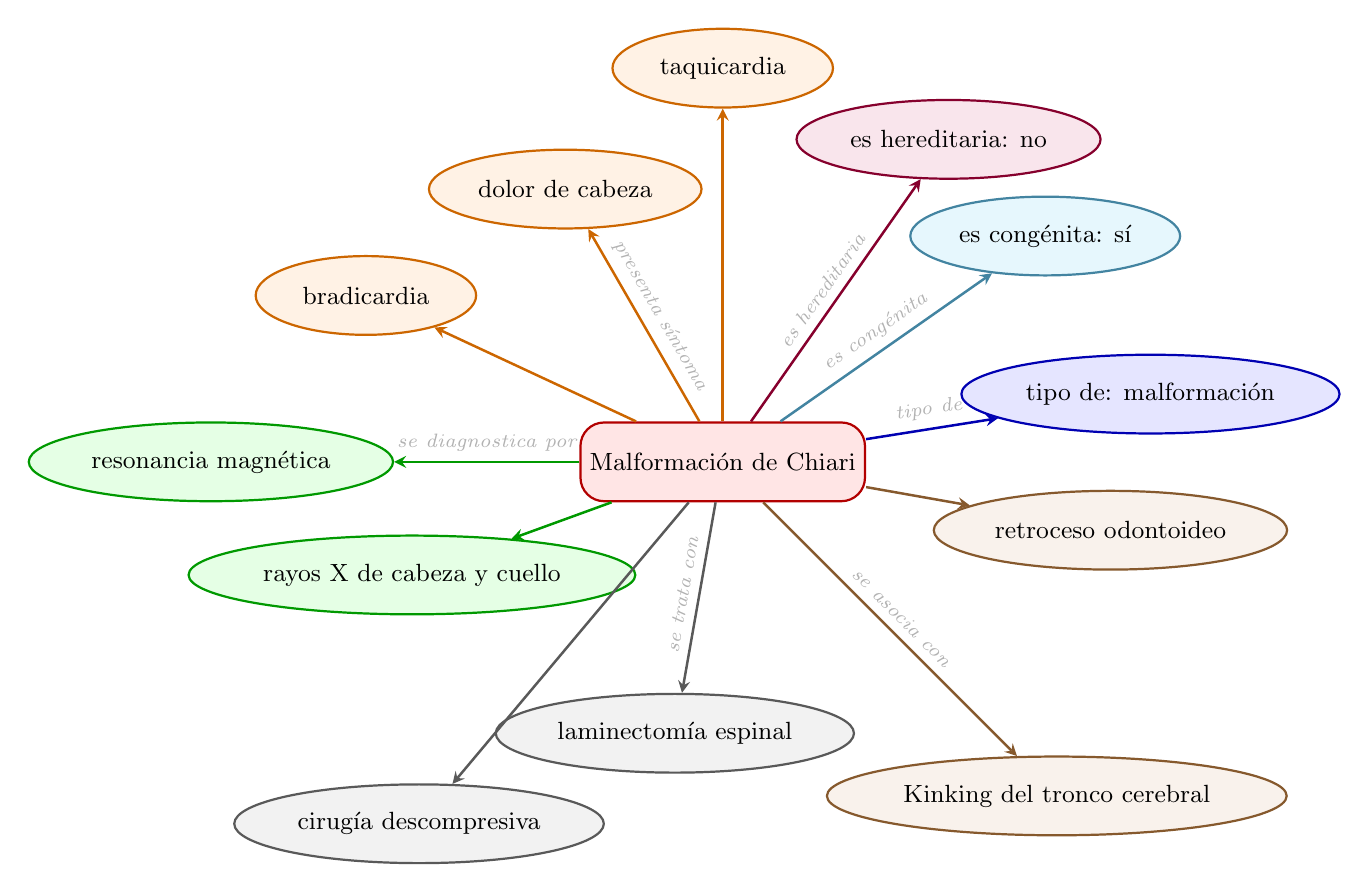
\begin{tikzpicture}[
    font=\small,
    node distance=3cm,
    main/.style={rectangle, rounded corners=3mm, draw=red!70!black, fill=red!10,
                 thick, minimum width=3.5cm, minimum height=1cm, align=center},
    entity/.style={ellipse, draw=gray!70, thick, minimum width=2.8cm, minimum height=1cm, align=center},
    arrow/.style={->, >=stealth, line width=0.9pt, rounded corners},
    relationlabel/.style={font=\scriptsize\itshape, text=gray!60, midway, sloped, above},
    % Colores por tipo de relación
    sintoma/.style={draw=orange!80!black, fill=orange!10},
    diagnostico/.style={draw=green!60!black, fill=green!10},
    tratamiento/.style={draw=gray!70!black, fill=gray!10},
    asociacion/.style={draw=brown!70!black, fill=brown!10},
    tipo/.style={draw=blue!70!black, fill=blue!10},
    herencia/.style={draw=purple!70!black, fill=purple!10},
    cong/.style={draw=cyan!60!black, fill=cyan!10}
]

% --- Nodo central ---
\node[main] (chiari) {Malformación de Chiari};

% --- Distribución radial de nodos ---
\node[entity, sintoma] (dolor) at (120:4) {dolor de cabeza};
\node[entity, sintoma] (bradi) at (155:5) {bradicardia};
\node[entity, sintoma] (taqui) at (90:5) {taquicardia};

\node[entity, diagnostico] (rm) at (180:6.5) {resonancia magnética};
\node[entity, diagnostico] (rx) at (200:4.2) {rayos X de cabeza y cuello};

\node[entity, tratamiento] (cirugia) at (230:6) {cirugía descompresiva};
\node[entity, tratamiento] (laminectomia) at (260:3.5) {laminectomía espinal};

\node[entity, asociacion] (kinking) at (315:6) {Kinking del tronco cerebral};
\node[entity, asociacion] (retroceso) at (350:5) {retroceso odontoideo};

\node[entity, herencia] (hereditaria) at (55:5) {es hereditaria: no};
\node[entity, cong] (congenita) at (35:5) {es congénita: sí};
\node[entity, tipo] (tipo) at (9:5.5) {tipo de: malformación};

% --- Flechas con etiquetas ---
\draw[arrow, orange!80!black] (chiari) -- (dolor) node[relationlabel] {presenta síntoma};
\draw[arrow, orange!80!black] (chiari) -- (bradi);
\draw[arrow, orange!80!black] (chiari) -- (taqui);

\draw[arrow, green!60!black] (chiari) -- (rm) node[relationlabel] {se diagnostica por};
\draw[arrow, green!60!black] (chiari) -- (rx);

\draw[arrow, gray!70!black] (chiari) -- (cirugia);
\draw[arrow, gray!70!black] (chiari) -- (laminectomia) node[relationlabel] {se trata con};

\draw[arrow, brown!70!black] (chiari) -- (kinking) node[relationlabel] {se asocia con};
\draw[arrow, brown!70!black] (chiari) -- (retroceso);

\draw[arrow, purple!70!black] (chiari) -- (hereditaria) node[relationlabel] {es hereditaria};
\draw[arrow, cyan!60!black] (chiari) -- (congenita) node[relationlabel] {es congénita};
\draw[arrow, blue!70!black] (chiari) -- (tipo) node[relationlabel] {tipo de};
\end{tikzpicture}

\caption{Grafo de relaciones principales de la entidad \textbf{Malformación de Chiari}.}
\end{figure}

\begin{figure}[h]
\centering
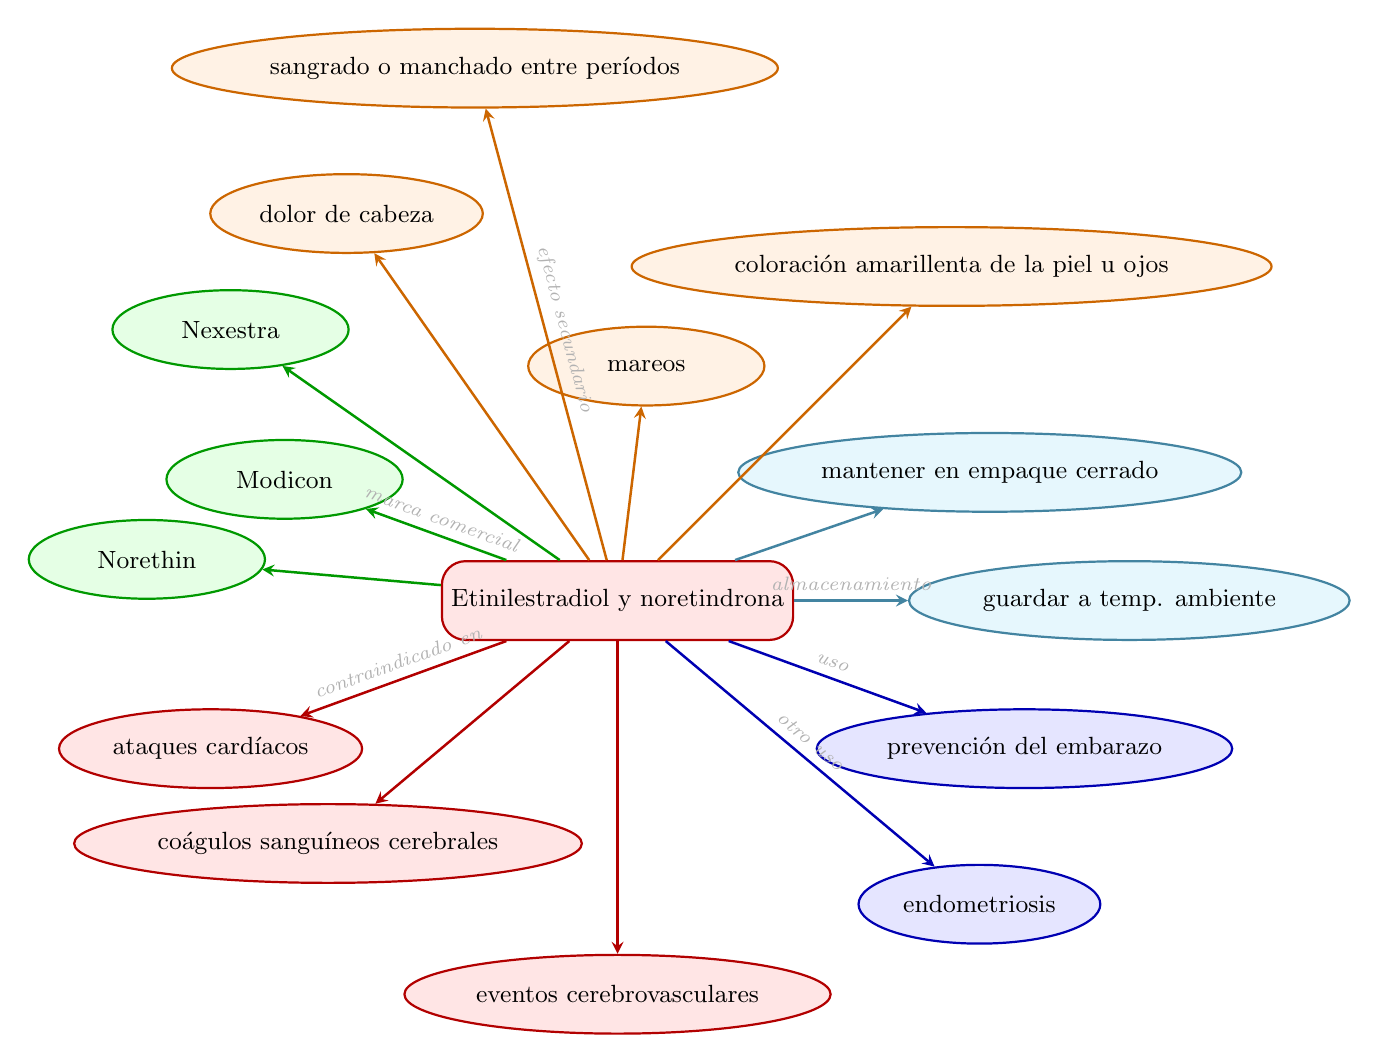
\begin{tikzpicture}[
    font=\small,
    node distance=3cm,
    main/.style={rectangle, rounded corners=3mm, draw=red!70!black, fill=red!10,
                 thick, minimum width=4cm, minimum height=1cm, align=center},
    entity/.style={ellipse, draw=gray!70, thick, minimum width=3cm, minimum height=1cm, align=center},
    arrow/.style={->, >=stealth, line width=0.9pt, rounded corners},
    relationlabel/.style={font=\scriptsize\itshape, text=gray!60, midway, sloped, above},
    % Colores por tipo de relación
    efecto/.style={draw=orange!80!black, fill=orange!10},
    contra/.style={draw=red!70!black, fill=red!10},
    marca/.style={draw=green!60!black, fill=green!10},
    uso/.style={draw=blue!70!black, fill=blue!10},
    almacen/.style={draw=cyan!60!black, fill=cyan!10},
    trata/.style={draw=teal!70!black, fill=teal!10},
    sobre/.style={draw=purple!70!black, fill=purple!10}
]

% --- Nodo central ---
\node[main] (med) {Etinilestradiol y noretindrona};

% --- Distribución radial de nodos ---
\node[entity, efecto] (sangrado) at (105:7) {sangrado o manchado entre períodos};
\node[entity, efecto] (dolor) at (125:6) {dolor de cabeza};
\node[entity, efecto] (mareo) at (83:3) {mareos};
\node[entity, efecto] (piel) at (45:6) {coloración amarillenta de la piel u ojos};

\node[entity, contra] (ataques) at (200:5.5) {ataques cardíacos};
\node[entity, contra] (coagulos) at (220:4.8) {coágulos sanguíneos cerebrales};
\node[entity, contra] (ictus) at (270:5) {eventos cerebrovasculares};

\node[entity, marca] (modicon) at (160:4.5) {Modicon};
\node[entity, marca] (norethin) at (175:6) {Norethin};
\node[entity, marca] (nexestra) at (145:6) {Nexestra};

\node[entity, uso] (prevencion) at (340:5.5) {prevención del embarazo};
\node[entity, uso] (endo) at (320:6) {endometriosis};

\node[entity, almacen] (temp) at (0:6.5) {guardar a temp. ambiente};
\node[entity, almacen] (empaque) at (19:5) {mantener en empaque cerrado};

% --- Flechas con etiquetas ---
\draw[arrow, orange!80!black] (med) -- (sangrado) node[relationlabel] {efecto secundario};
\draw[arrow, orange!80!black] (med) -- (dolor);
\draw[arrow, orange!80!black] (med) -- (mareo);
\draw[arrow, orange!80!black] (med) -- (piel);

\draw[arrow, red!70!black] (med) -- (ataques) node[relationlabel] {contraindicado en};
\draw[arrow, red!70!black] (med) -- (coagulos);
\draw[arrow, red!70!black] (med) -- (ictus);

\draw[arrow, green!60!black] (med) -- (modicon) node[relationlabel] {marca comercial};
\draw[arrow, green!60!black] (med) -- (norethin);
\draw[arrow, green!60!black] (med) -- (nexestra);

\draw[arrow, blue!70!black] (med) -- (prevencion) node[relationlabel] {uso};
\draw[arrow, blue!70!black] (med) -- (endo) node[relationlabel] {otro uso};

\draw[arrow, cyan!60!black] (med) -- (temp) node[relationlabel] {almacenamiento};
\draw[arrow, cyan!60!black] (med) -- (empaque);

\end{tikzpicture}
\caption{Grafo de relaciones principales de la entidad \textbf{Etinilestradiol y noretindrona}.}
\end{figure}


\begin{figure}[h]
\centering
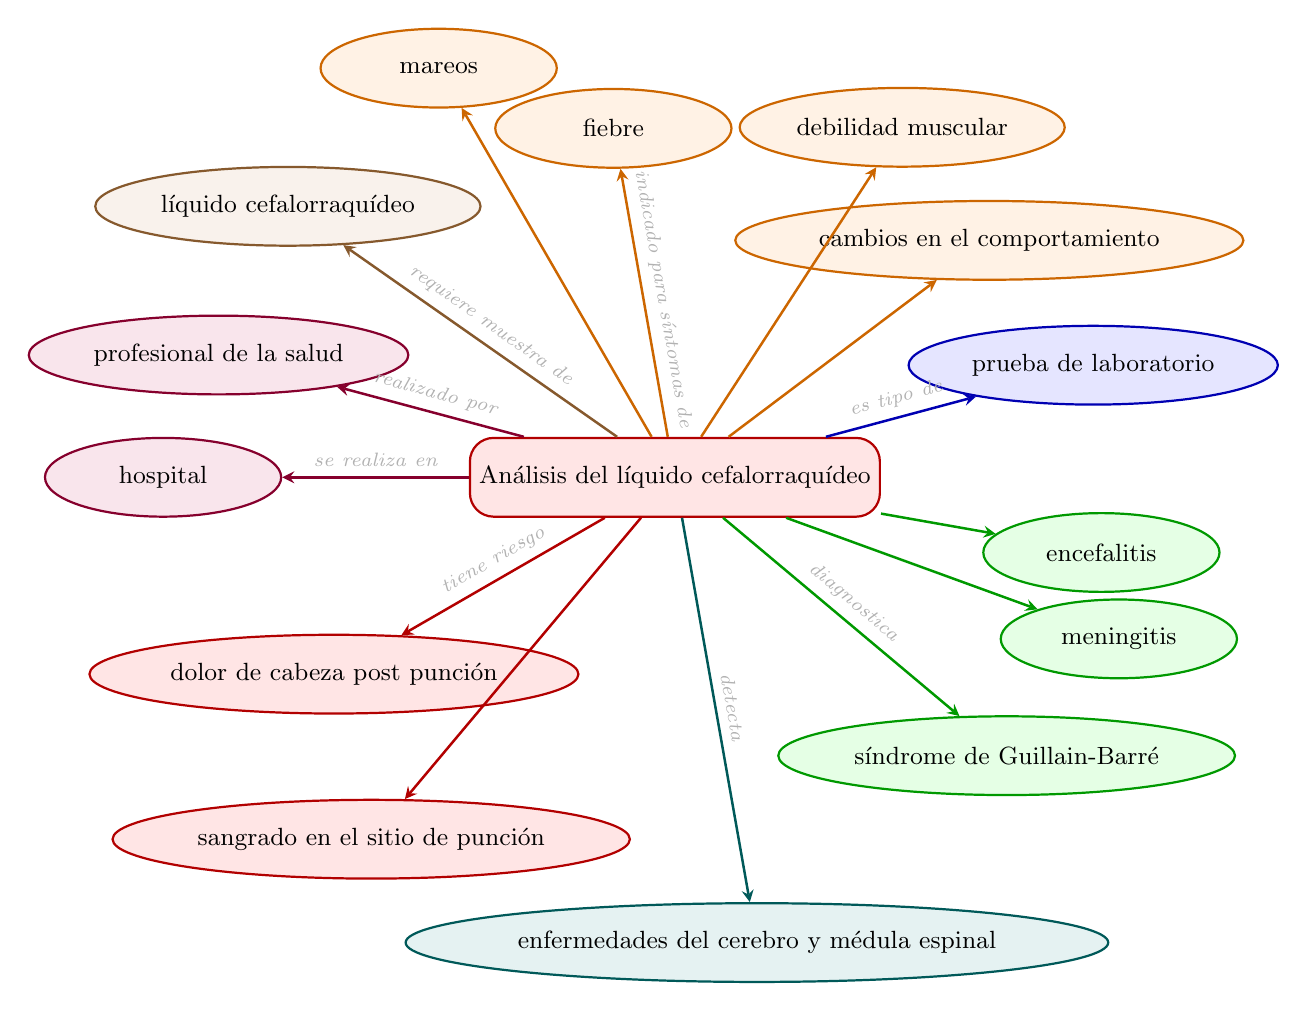
\begin{tikzpicture}[
    font=\small,
    node distance=3cm,
    main/.style={rectangle, rounded corners=3mm, draw=red!70!black, fill=red!10,
                 thick, minimum width=4cm, minimum height=1cm, align=center},
    entity/.style={ellipse, draw=gray!70, thick, minimum width=3cm, minimum height=1cm, align=center},
    arrow/.style={->, >=stealth, line width=0.9pt, rounded corners},
    relationlabel/.style={font=\scriptsize\itshape, text=gray!60, midway, sloped, above},
    % Colores por tipo de relación
    indicado/.style={draw=orange!80!black, fill=orange!10},
    tipo/.style={draw=blue!70!black, fill=blue!10},
    diagnostica/.style={draw=green!60!black, fill=green!10},
    detecta/.style={draw=teal!70!black, fill=teal!10},
    riesgo/.style={draw=red!70!black, fill=red!10},
    realiza/.style={draw=purple!70!black, fill=purple!10},
    muestra/.style={draw=brown!70!black, fill=brown!10}
]

% --- Nodo central ---
\node[main] (analisis) {Análisis del líquido cefalorraquídeo};

% --- Distribución radial de nodos ---
\node[entity, indicado] (fiebre) at (100:4.5) {fiebre};
\node[entity, indicado] (mareos) at (120:6) {mareos};
\node[entity, indicado] (debilidad) at (57:5.3) {debilidad muscular};
\node[entity, indicado] (comportamiento) at (37:5) {cambios en el comportamiento};

\node[entity, tipo] (prueba) at (15:5.5) {prueba de laboratorio};

\node[entity, diagnostica] (encefalitis) at (350:5.5) {encefalitis};
\node[entity, diagnostica] (guillian) at (320:5.5) {síndrome de Guillain-Barré};
\node[entity, diagnostica] (meningitis) at (340:6) {meningitis};

\node[entity, detecta] (enfermedades) at (280:6) {enfermedades del cerebro y médula espinal};

\node[entity, riesgo] (dolorpun) at (210:5) {dolor de cabeza post punción};
\node[entity, riesgo] (sangrado) at (230:6) {sangrado en el sitio de punción};

\node[entity, realiza] (profesional) at (165:6) {profesional de la salud};
\node[entity, realiza] (hospital) at (180:6.5) {hospital};

\node[entity, muestra] (liquido) at (145:6) {líquido cefalorraquídeo};

% --- Flechas con etiquetas ---
\draw[arrow, orange!80!black] (analisis) -- (fiebre) node[relationlabel] {indicado para síntomas de};
\draw[arrow, orange!80!black] (analisis) -- (mareos);
\draw[arrow, orange!80!black] (analisis) -- (debilidad);
\draw[arrow, orange!80!black] (analisis) -- (comportamiento);

\draw[arrow, blue!70!black] (analisis) -- (prueba) node[relationlabel] {es tipo de};

\draw[arrow, green!60!black] (analisis) -- (guillian) node[relationlabel] {diagnostica};
\draw[arrow, green!60!black] (analisis) -- (meningitis);
\draw[arrow, green!60!black] (analisis) -- (encefalitis);

\draw[arrow, teal!70!black] (analisis) -- (enfermedades) node[relationlabel] {detecta};

\draw[arrow, red!70!black] (analisis) -- (dolorpun) node[relationlabel] {tiene riesgo};
\draw[arrow, red!70!black] (analisis) -- (sangrado);

\draw[arrow, purple!70!black] (analisis) -- (profesional) node[relationlabel] {realizado por};
\draw[arrow, purple!70!black] (analisis) -- (hospital) node[relationlabel] {se realiza en};

\draw[arrow, brown!70!black] (analisis) -- (liquido) node[relationlabel] {requiere muestra de};

\end{tikzpicture}
\caption{Grafo de relaciones principales de la entidad \textbf{Análisis del líquido cefalorraquídeo}.}
\end{figure}


\end{document}
